%
% TU/e Style Master Thesis template for LaTeX
%
% Public version 1.0
% 2010 - 2013 Thijs Nugteren and Joos Buijs
%
% THIS IS THE MAIN FILE (i.e. compile this file, compiling the others directly won't work)
%
\documentclass[a4paper,10pt,twoside]{report}

%all the other includes etc. are done in the thesis.sty file.
\usepackage{thesis}

%
% These commands need to be defined in order to produce a correct and personalized document
%
\newcommand{\shortdoctitle}{}
\newcommand{\doctitle}{Behavior Analysis of Elderly using Topic Models}
\newcommand{\docsubtitle}{Master Thesis of}

\newcommand{\me}{Kristin Rieping}
\newcommand{\keywords}{keyword1, keyword2, keyword3}
\newcommand{\version}{}
\newcommand{\monthYear}{August 2013}

%Be sure to use all the titles for your committee members!!! (their names show up on the very first page!)
\newcommand{\firstCommitteeMember}{Prof. Dr. ir. B.J.A. Kr\"{o}se}
\newcommand{\secondCommitteeMember}{Dr. G. Englebienne}

\author{\me}

%
% PDF settings
%
\hypersetup
{
    pdfauthor={\me},
    pdftitle={\shortdoctitle},
    pdfsubject={\doctitle},
    pdfkeywords={\keywords}
}

\begin{document}

%use this include for PDF and distribution versions
\pagenumbering{roman}
\begin{titlepage}
\begin{center}

\includegraphics[height=2cm]{figures/logo-UvA-wide}\\
%\LARGE
%Eindhoven University of Technology \\
\large
Faculty of Science \\
Master Artificial Intelligence\\
Track Intelligent Systems


\vspace*{10cm}

\setlength{\TPHorizModule}{1mm}
\setlength{\TPVertModule}{\TPHorizModule}
% Set the Paragraph Indent to zero, so the first line is not Indented
% Back-up the current value so it can be put back at the end of the title page
\newlength{\backupparindent}
\setlength{\backupparindent}{\parindent}
\setlength{\parindent}{0mm}			
% Begins a textbox at 72 mm from the left of the edge of the paper and 89 mm from the top
% The width of the textbox is 95 mm (167 - 72 mm)
% The height of the box cannot be defined, so it is your task to keep the text not too long
\begin{textblock}{120}(47,89)
    \vspace*{1mm}
    \huge
    \textbf{\doctitle \\}
    \Large
    \vspace*{5mm}
    \textit{\docsubtitle}\\
    \vspace*{10mm}
    \Large
    \me\\
\end{textblock}

\large
Supervisors:\\
\begin{tabular}{rl}
    \firstCommitteeMember\\
    \secondCommitteeMember\\
    \thirdCommitteeMember\\
\end{tabular}

\vfill
\version

\vfill
%\docdate \\
\large
Amsterdam, \monthYear\\

% Put the Paragraph Indent back to its original value
\setlength{\parindent}{\backupparindent}
\end{center}
\end{titlepage} 

\normalsize

\clearemptydoublepage

%Sometimes line numbers are nice, uncomment the next line to enable:
%\linenumbers

%It could be handy to have a list of todos and brainstorms in your thesis
%\chapter*{*General todos*}\todo{remove this chapter}
%\input{chapters/general_todos}

%\chapter*{*Brainstorm results*}\todo{remove this chapter}
%\input{chapters/brainstorm_results}

\chapter*{Abstract}\label{chapter:abstract}
In this thesis two novel variations of the Latent Dirichlet Allocation (LDA) model are presented. The models give the opportunity to detect patterns in multi-dimensional data in an unsupervised manner. LDA-Gaussian is a combination of a Gaussian Mixture Model and a LDA model. Here the multinomial distribution of the topics, that is normally used in the LDA model, is replaced by a set of Gaussian Distributions. In this way similar looking sensor data is automatically grouped together and captured in the same topic.
LDA-Poisson, the second variation of the model, takes a set of Poisson Distribution for the topic descriptions. This distribution makes it possible to handle discrete multi-dimensional data. The parameters of both models are determined with an EM-algorithm.
Both models are applied to real sensor data, which is gathered in the homes of elderly people. It is shown that meaningful topics can be found and that a semantic description of these topics can be given.

\clearemptydoublepage

%An executive summary if you want:
%\chapter*{Executive summary}\label{chapter:executive_summary}
%\input{chapters/executive_summary}

%\clearemptydoublepage


% \chapter*{Preface}\label{chapter:preface}
% Please write all your preface text here. If you do so, don't forget to thank your supervisor, other committee members, your family, colleagues etc.\ etc. 
% 
% \clearemptydoublepage

\tableofcontents

\clearemptydoublepage

\listoffigures

% \clearemptydoublepage
% 
% \listoftables
% 
% \clearemptydoublepage
% 
% \lstlistoflistings

\clearemptydoublepage

\chapter{Introduction}\label{chapter:introduction}
\setcounter{page}{0}
\pagenumbering{arabic}
%from here on, start the 'real' page numbering, from 1, with normal digits
%NOG DOEN:
% 

%START
The life expectancy of people is assumed to rise continuously in the following years \cite{UnitedNations}. As a consequence the percentage of elderly increases. Elderly people often need more health care but studies show that they prefer to live at home \cite{Cavallo:1315167}. The manpower to take care of elderly people is not always available. That is why monitoring the health condition of people in their home environment becomes more and more important. In this way slowly emerging declines in the health condition of people can be detected and appropriate health care can be granted if it is necessary before critical health conditions are reached.\\

%Monitoring elderly
New systems give the possibility to monitor elderly from the distance or even automatically \cite{Tamura1998573}. Different systems give the possibility to detect accidents or monitor the health condition on a long time basis. Some systems still need the action of a person involving into the system. For example the inhabitant has to push a button if an accident occurs \cite{Kwon20125774}. Other systems use cameras to monitor the elderly \cite{Mubashir2013144,Nagai2010204}. But these methods are privacy-sensitive and often not adopted by the elderly.\\

%Pervasive sensors
Less intrusive methods use simple sensors like motion sensors or pressure mats that are placed in the homes of people \cite{Tapia04activityrecognition,4912776}. Extracting valuable information out of this data is however difficult and that is why activity recognition is often done to make the data more easily to interpret. Different techniques attempt to extract `Activities of daily living' (ADL's). Changes in the ADL's can be a sign for declines of peoples health \cite{Tapia04activityrecognition}.
Some researchers depend on annotated data to find ADL's in sensor data \cite{Tapia04activityrecognition,Hong2009236,Wilson:2005:STA:2154273.2154280}. But the task of labeling the data is time consuming and also intrusive, if the labeling is done by a different person. The knowledge of being observed by a sensor, for example a camera, might change the behavior patterns of a person and in this way the data is not accurate. Annotation that is done by the subject himself also might not be accurate, because the person has to interrupt his daily behavior to write down the annotation of the activities.\\

% unsupervised topic models on sensor data, wat is al gedaan
A way to automatically find behavior patterns in sensor data is by applying a topic model to the data. Topic models are initially designed for classifying text documents and they are able to find abstract topics, such as `politics', `sports', `finances' etc. But a number of researchers have applied the topic model `Latent Dirichlet Allocation' (LDA) to different kind of sensor data \cite{farrahi2008daily,journals/percom/ChikhaouiWP12}. The found topics are comparable to ADL's and can give a good representation of peoples daily behavior.
There is however a mayor difference between textual and sensor data. In the LDA model presented by Blei \cite{blei2003latent} the documents are represented by a Bag-of-words (BOW). A BOW model is an unordered representation of words, that does not take the grammar or the order of the words into account.\\

% Hoe kan LDA worden toegepast.
To make use of the LDA model on sensor data one has to create artificial words. There are numerous ways ways to create words from sensor data.
Some researchers create artificial words by quantizing the data and adding a time-value. The BOW representation then directly is used on these 'words'\cite{farrahi2008daily,EXSY:EXSY12033}. This approach requires a large dictionary of words to find behavior patterns in the data, to be able to capture all the variations in artificial words. Other researchers first cluster the data and then apply the LDA model \cite{Huynh:2008:DAP:1409635.1409638,Casale:2009}. In this way the size of the dictionary is smaller and less data is required.  But finding the correct clusters is however difficult.\\

% mijn bijdrage
In this thesis the two new topic models `LDA-Gaussian' and `LDA-Poisson' are developed. These models are able to capture similar observations/words into the same topic automatically. The clustering and the LDA model are combined into one model and except for the construction of the artificial words, no further pre-processing is necessary .
In the original LDA model (Blei) the topics are described by a multinomial distribution over the words of the vocabulary. In the `LDA-Gaussian' model this distribution is replaced with a Gaussian distribution, so that similar words are caught in the same topic. `LDA-Poisson' is a variation on this model, where the underlying distribution is Poisson. In this way event based sensor data can be modeled.
The parameters of both models are found with an Expectation-Maximalization-procedure (EM-procedure), which uses the likelihood of the model to converge to the optimal model parameters. No pre-processing of the data is needed except for the quantization. The models are applied on real sensor data, that is obtained from the houses of solitary living elderly. 
All sensors are binary and are experienced as non-intrusive by the inhabitants. These elderly people live in a care home and get health care on a regular basis. Still they are able to live on their own.\\


% START outline verslag
In the next chapter of this thesis an overview of related approaches are given. In chapter \ref{chapter:data_description} the data that is used is described in more detail and after that representation of the features is given in chapter \ref{chapter:features}. This chapter is followed by chapter \ref{chapter:topic_models} which introduces the `LDA-Gaussian' and `LDA-Poisson' models. Chapter \ref{chapter:experiments} contains the different experiments that are performed on the available data. In chapter \ref{chapter:conclusions} the conclusions of this thesis is presented and some suggestions for future work are given.




\clearemptydoublepage

\chapter{Related Work}\label{chapter:related_work}
% INTRODUCTION and HEALTH MONITORING
The goal of monitoring the health of people is to detect accidents or even more important to prevent accidents and critical health conditions. Changes in the daily behavior patterns can be a sign of changes in the health of people. This can be both mental or physical declines.
There are different ways to monitor the health condition of people. Cameras or microphones can be very useful to monitor peoples behavior \cite{Nagai2010204, Wu_2003_4676}, but these sensors are invading the privacy of people and often not accepted as sensors in peoples homes.\\

% PERVASIVE SENSOR SYSTEMS SUPERVISED
Simple binary sensors such us motion sensors, contact switches or pressure mats are preferable for health monitoring in home environments. These sensors are low in cost and easy to install. Moreover, they are also experienced as non-intrusive and not disturbing by the inhabitants. Numerous researchers implemented different approaches to apply activity recognition on data generated by these kind of sensors. These activities and especially changes in these activities, often referred to as ADL's, can then give valuable information on peoples health \cite{journals/hf/RogersMWF98}.
% Tapia
Tapia et al. \cite{Tapia04activityrecognition} uses a naive Bayes classifier to find activities in annotated, sensor data. They show that it is possible to find activities in ubiquitous, simple sensor data, that was obtained in real-life environments.
% Kasteren
In the work of Kasteren et al. \cite{vanKasteren:2008:AAR:1409635.1409637} two approaches for recognizing activities in sensor data are compared. The Hidden Markov Model and the Conditional Random Field are both applied to annotated, real-life sensor data. They also vary between different kind of sensor readings and show that this can improve the results for recognizing activities with their approaches.
% Wilson
Wilson et al. \cite{Wilson:2005:STA:2154273.2154280} implemented a Particle Filter to find activities in simulated as well as real-life data. They are able to distinguish the actions between multiple people in the environment.
% Hong
Hong et al. \cite{Hong2009236} uses ontologies to describe daily activities. They use an evidential network to describe activities in a hierarchical way.
\\


% UNSUPERVISED USAGE OF LDA
All of the previous approaches used annotated data. Generating this labeled data is however difficult, time consuming and the determined labels are not always accurate. For this reason supervised methods are preferred above supervised methods in this field.
Various authors applied LDA to different kind of data. This topic model is able to find abstract descriptions of activities in data automatically.\\

% Chikhaoui
Chikhaoui et al. \cite{journals/percom/ChikhaouiWP12} uses the topic model LDA in combination with sequential pattern mining to find activities in various datasets. The sequential pattern are used as words, which are the input for the LDA model.  They test their method on varied annotated data sets. The topics that are found describe activities and the accuracy is measured by comparing the topics with annotation labels. In their work the focus lays on detecting activities and not so much on the global idea of detecting behavior patterns as it is done in this work.\\

% Huynh, Casale
Huyhn et al. \cite{Huynh:2008:DAP:1409635.1409638} and Casale et al. \cite{Casale:2009} both try to discover daily routines from sensor data. Acceleration sensors that are attached to the human body generate a continuous stream of data. The data is quantized in different time intervals and in this ways artificial words are created. The dictionary, which contains all unique words, is quite big, because small variations in the sensor data generates different words. Therefore the authors cluster the data on forehand with the k-means algorithm. In this way the size of the dictionary can be reduced. The choice of $k$ however is of big influence on the outcome of the LDA model. That is why in this thesis a different approach is used to handle the big amount of variations in the artificial words.\\

%that is obtained from acceleration sensors which are attached to the human body. They first create artificial words by clustering the data and than apply LDA to these words. The clustering is necessary to reduce the size of the dictionary.

% 
% In this way the reduce the size of the vocabulary. This is necessary because otherwise there are to many dimensions and to less data.
% 
% waarom moeten ze het clusteren van te voren? 
% 
% by applying LDA to sensor data obtained from acceleration sensors that are attached to the body.
% daily routines
% 
% From acceleration features, that are clustered in advance, they generate the artificial words. The clustering is necessary to group similar words together. In this way the size of the dictionary is reduced and LDA can find meaningful topics in the data. Choosing the amount of clusters on forehand is however difficult and has a big influence on the outcome of the LDA model.\\
% 
% Lukt het hun wel om zinvolle topics te creeren en als ja hoe?

% % Phung DOEN
% Phung et al. \cite{PhungATVK09} applys LDA to data that is gained of a WiFi network. They find behavior patterns of people in their work environment.\\

% Farrahi DUIDELIJKER
Farrahi et al. \cite{farrahi2008daily} applies LDA to location data gained from cell information of mobile phones. A lot of data is available and artificial words are created by combining the location of a person at three consecutive time steps and adding the time value. In this way every time of a day is described with a word. This approach of dividing a day into words is also adopted in this thesis. In Farrahi's work only 512 different words are possible, but about 2800 days of 68 different people are available. This ratio of vocabulary size and available data makes their approach a successful way to find latent topics in location data, without the need of clustering the data on forehand. Their way of describing the features is a good option to capture transitions in locations.\\

% Castanedo
In the work of Castanedo et al. \cite{EXSY:EXSY12033} they also apply the LDA model on sensor data without pre-clustering the dictionary. For their work much data was available, which was obtained in an office environment. The words are however represented differently than it is done in the work of Farrahi et al. Not every time of a day is divided into words, but only time periods that contain sensor activations build the artificial words. They indicate that it can become difficult to give a good interpretation of the topics, that are found. So it is questionable if leaving out time periods without sensor activations in the feature representation leads to a better result.\\







\clearemptydoublepage

\chapter{Data}\label{chapter:data_description}
In this chapter a description of the houses and the inhabitants is given. The different kind of sensors are explained and an impression of the received data is given.

\section{Homes and persons}
In the homes of five different people sensors are installed. The floor-plan of these homes is for all residents the same and is shown in figure \ref{fig:floorplan}. There might be small differences of the locations of the sensors due to the personal arrangements of peoples personal belongings.
The persons that live in the homes are people that need healthcare on a regular basis, they are further able to live on their own. The amount of data collected differs for the different houses, but there is at least 63 days of data available for every house. An overview of the different houses is given in table \ref{table:houses}

\begin{figure}
\centering
 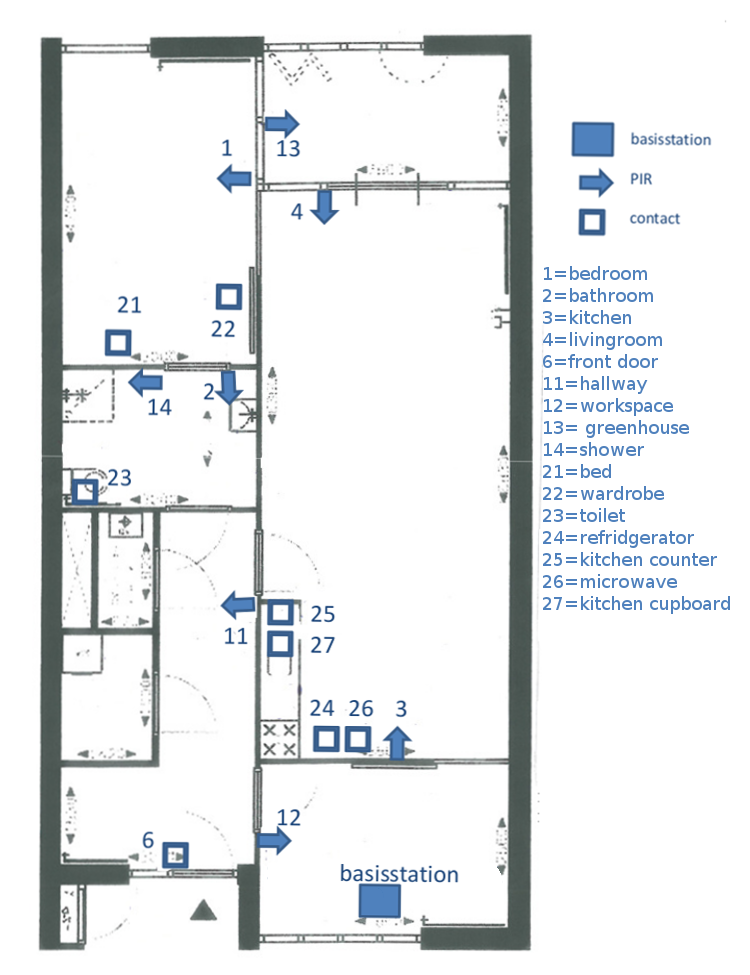
\includegraphics[width=0.7\textwidth]{Pictures/floorplan.png}
 \caption{Floorplan of the houses with sensor descriptions}
 \label{fig:floorplan}
\end{figure}


\begin{table}[h]
\centering
\begin{tabular}{lccccc}
\centering
HouseNr & 1 & 2 & 3 & 4 & 5 \\
\hline
\# of days & 142 & 98 & 89 & 63 & 73 \\
%time period \\
mean activities per day & 488 & 523 & 668 & 565 & 427 \\
\end{tabular}
\caption{ }
\label{table:houses}
\end{table}




\section{Sensors}
There are different types of sensors installed in the homes. The contact switches are mostly installed at doors and cupboards. They get the value 'one' if a door is opened and the value 'zero' if the door is closed again.
The motion-sensor (PIR) are placed at different places in the homes, mostly against the walls. They have a range of 5 meters. If a motion occurs in the region the sensor sends an impulse value, which means that the value becomes 'one' and immediately 'zero' again . After that the sensor is set to mute for about 3 minutes, which means that in this time there is no motion captured. In this way constantly firing of the sensor will be avoided. The sensor system is active 24 hours and 7 days a week. However failure can occur due to network problems, sensor failing or other unexpected problems.

\section{Received Data}
In figure \ref{fig:PlaineSensorData} the data stream of two different hours of one day is shown. The data belongs to one person. Several sensors that are located in the same room are manually grouped together in a field. The fields are $\{$'kitchen', 'living room', 'bathroom', 'bedroom', 'hallway'$\}$. They are marked in the figure with different colors.

\begin{figure}[h!]
   \centering
   \begin{minipage}[b]{0.45\textwidth}
     \centering
     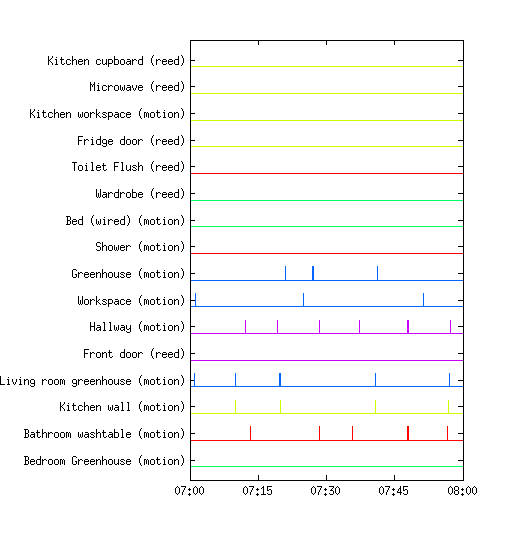
\includegraphics[width=\textwidth]{Pictures/SensorsMorningHN3Day34.png}
   \end{minipage}
   ~
   \begin{minipage}[b]{0.45\textwidth}
     \centering
     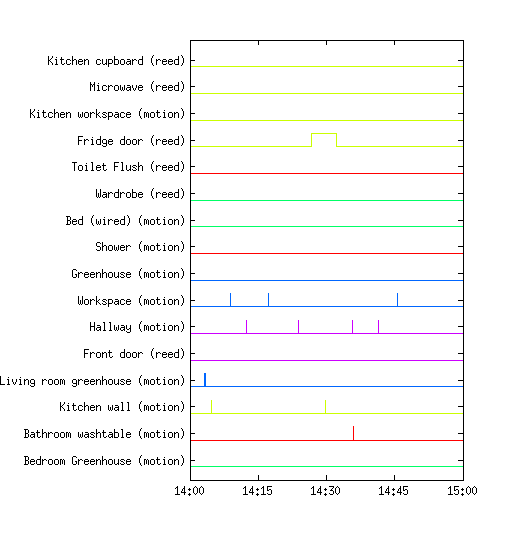
\includegraphics[width=\textwidth]{Pictures/SensorsNoonHN3Day34.png}
   \end{minipage}
   \caption{Sensor Data for two different hours at a day of one person. The fields `kitchen`,'living room','bathroom','bedroom','hallway' are marked with the colors 'yellow', 'blue', 'red', 'green', 'purple' respectively.}
   \label{fig:PlaineSensorData}
 \end{figure}

In the figure one can see the different type of data that is generated by the different sensor types. The fridge sensor is a reed sensor which has the value '1' for a longer period of time, when the door is opened for a while. The motion sensors on the other hand only give a impulse value as mentioned before. Some sensors are not triggered at all in the time intervals that are shown.


\clearemptydoublepage

\chapter{Features}\label{chapter:features}
The data that is received from the sensors generates a continuous data stream for every sensor. A good feature representation of the data is required so that the LDA model can be applied. The feature representation that is described in this chapter is used as the artificial words for the LDA model that is described in chapter \ref{chapter:topic_models} about the Topic model.
First the data is divided into five fields and all the sensors in one field are grouped together. In this way the data is reduced to five dimensions. 
The continuous data stream cannot be used as input for the LDA model. Like it is done in the work of Farrahi \cite{farrahi2008daily} the data of one day is divided into time-slices of length $l$. If for example the length of the time-slices is $l=30$ min., the number of time-slices on one day is $n=48$. For a chosen number of the time-slices $n$ the length of time-slices for one day can then be calculated with $l=1440/n$ in minutes. In the experiments (chapter \ref{chapter:experiments}) the number of time-slices is varied to see the effect on the topic model.
A day starts and ends at 3 a.m. in the morning. In this way the chance to cut between activities is reduced. It still can occur that a person goes to bed late or that he needs to visit the toilet. For now this fact is left out in the part of modeling.\\

For every time-slice the number of sensor activations of one field are counted. In one time-slice for each sensor field the number of times is counted that the signal changes from zero to one. The duration of an active signal, thus for how long a sensor field has the value one, is not taken into account. This is done because for example a door that accidentally is left open would otherwise generate a high value although this value is not very informative and would though disturb the data. Then the observations contains a high value but does not contain a lot of information about the behavior.
Every sensor field then builds a dimension of the observations $o_n$. In figure \ref{fig:FeatEx} an example on how the data is translated into a vector representation is given for one time-slice.

\begin{figure}[h]
\centering
\begin{minipage}{0.55\linewidth}
\centering
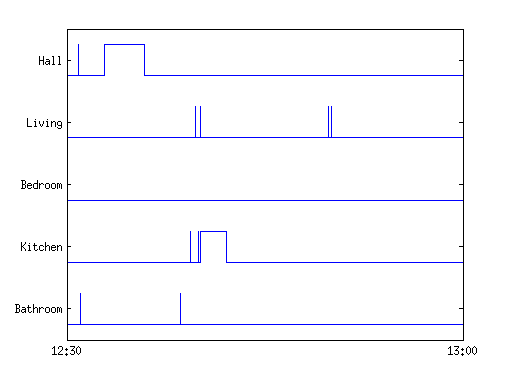
\includegraphics[width=\textwidth]{Pictures/FeatExample.png}
\label{fig:FeatEx}
\end{minipage}
\begin{minipage}{0.35\linewidth}
\centering
\begin{equation*}
o_n = 
 \begin{bmatrix} 
 o_{Hall}\\
 o_{Living}\\
 o_{Bedroom}\\
 o_{Kitchen}\\
 o_{Bathroom}\\
 o_{time}
 \end{bmatrix}
 =
  \begin{bmatrix} 
 2\\
 4\\
 0\\
 3\\
 2\\
 t
 \end{bmatrix}
\end{equation*}
\end{minipage}
\caption{Vector representation of the data. The data of the sensors is shown in the left image. It is translated in the vector shown on the right-hand side.}
\end{figure}

The last dimension of the observation $o_n$ represents the time value of the given time-slice. There are two different ways how the time dimension is added to the observations. The fine-grain representation adds the number of the time-slice in which an observations is captured, at the end of the observation vector. In the coarse-grain representation, which is also used in the work Farrahi \cite{} and Castanedo \cite{}, the 24 hours of a day are divided into the five time intervals $\{ 3am - 8am, 8am - 1pm, 1pm - 18pm, 18pm - 23pm, 23pm - 3am  \}$. So the observation of figure \ref{fig:FeatEx} will become $o_n=\{2,4,0,3,2,2\}$ in the coarse-grain representation. The observation falls into the second time interval. In the fine-grain representation the observation will be $o_n=\{2,4,0,3,2,20\}$ if the total number of time-slices on a day is $n=48$.\\




If the number of time-slices is set to $n=48$ the maximal value that is observed in one field is 28. This is an extreme value and occurs not that often in the data. If the maximum value for each field is set to 15 and the time is coarse grain, there are approximately 4 million ($10^5*5$) possible observations that can be made. As a comparison: In the work of Farrahi \cite{} only 512 ($4^3*8$) different observations are possible and 2856 days of data for 68 people is available.\\
In table \ref{tab:features} an overview is given how many unique words are actual observed for the different houses and how many words are totally observed ($48*\text{\# of days}$). One can see that the number of unique observations scales with the number of days available for each house. This shows that there are a lot of unseen observations in the data.\\


\begin{table}
 \centering
 \begin{tabular}{l c c c c c}
  HouseNr & 1 & 2 & 3 & 4 & 5\\
  \hline
  \# of days & 142 & 98 & 89 & 63 & 73 \\
  words & 6816 & 4704 & 4272 & 3024 & 3504 \\
  unique words & 2147 & 1644 & 1764 & 1068 & 1087\\
 \end{tabular}
 \caption{}
 \label{tab:features}
\end{table}


The given feature representation, with the two variation of the time dimensions, fine grain and coarse grain, are used in the following chapters. There are much more possibilities to describe the feature. An overview of different possibilities is given in the Future work (chapter \ref{chapter:future_work}).

%Every field of the observation has a different distribution on how often an activity of the 
%In figure ... an overview of the distribution of the values of the five fields is shown. For house number one the observation 
% EVENTUEL nog histograms of one house toevoegen

\clearemptydoublepage

\chapter{Topic Models}\label{chapter:topic_models}
In the introduction of this section we describe the general idea of topic models followed by a section that describes how this kind of models can be used on the sensor data that we have. After that we introduce the extension of the LDA model which combines the clustering and topic estimation in one algorithm. And after that LDA-Poisson model is described.

\section{Introduction to Topic Models}
Topic models are often used in the field of document classification. Given a set of documents (corpus) it is assumed that every document belongs to one or more topic(s). So for example a news article may belong for some percentage, let us say 30 \%,  to the topic 'Economy' and for 70 \%  to the topic 'Politics'. Another document of the same Corpus may belong to the topic 'Economy' with 50 \%, 'Politics' with 30 \% and 'Global Warming' with 20 \%. There might be a lot of different topics and the topics can have different level of details. \\
The topics are defined by several words that can occur in the documents. The topic 'Economy' may be defined by the list of words \{'trade', 'industry','GDP'\}. Other topics have different lists of words that describe them. The list might be longer or shorter and the words in the list will depend on the corpus that is used to generate the topics. It might also be the case that one word belongs to multiple topics. Eventually we can find the topic distribution of a document according to the words that are included in this document.\\
In the topic model 'Latent Dirichlet Allocation' (LDA) it is assumed that a Corpus can be made out of a generative process. The parameters that generate the corpus are than used to describe the model of the corpus. The generative process which builds a corpus is as follows:\\
For every document that is generated in the Corpus
\begin{enumerate}
 \item Choose the amount of words in the document from $N \sim Possoin(\xi)$.
 \item Choose a topic distribution $\theta \sim Dir(\alpha)$ for the document.
 \item For each of the N words $w_n$:
 
 \begin{enumerate}
  \item Choose a topic $z_n \sim Multinomial(\theta)$.
  \item Choose a set of words $w_n$ from the set of all words $V$ from $p(o_n |z_n;\beta)$, a multinomial probability conditioned on the topic $z_n$. Where $\beta$ is the distribution over words given a topic.
 \end{enumerate}

\end{enumerate}

The model is also shown in figure~\ref{fig:modelBasic}. The parameters $\alpha$ and $\beta$ define a corpus.

\begin{figure}[h!]
\centering
\def\svgwidth{400pt}
\input{Pictures/ModelBasic.pdf_tex}
\caption{Graphical representation of the LDA model}
\label{fig:modelBasic}
\end{figure}

To determine the model parameters an EM-algorithm can be used. How this algorithm can be applied is extensively described in~\cite{blei2003latent}. \\
In the next section we describe how this model can be used with the sensor data, that is gained in the different houses.


\section{Topic models with Sensor Data}

In order to employ the topic model with the sensor data we first introduce the different levels of description given our data and relate them to the terms of document classification.
\begin{itemize}
 \item \textbf{Dataset/Corpus}: One dataset $C$ describes the sensor data that is gained in the home of a single person. So for every person there is a separate dataset. This set of data can be compared with a Corpus in document classification.
 \item \textbf{Day/Document}: Every Dataset is divided in days. A day can be compared with one document in a Corpus.
 \item \textbf{Observations/Words}: Finally every day is build of a set of observations. The amount and dimension of the observations depend on the representation of the features, which is described later in chapter \ref{sec:features}. Observations can be roughly compared with words in document classification.
\end{itemize}

There are some differences between the data that is used for topic detection in documents and our sensor data.\\
The main difference is that words that look similar to each other, like "illusion" and "allusion", may belong to a totally different topic in the document classification. But in our case, two observation that are similar to each other, are more likely to refer to the same topic. So for example if the topic "preparing food" has the observation using fridge 3 times in it, an observation of using fridge 4 times may also refer to the same topic. That is why we cannot directly compare the words in a text document with the observations used in the sensor data.\\
Another difference is that in the topic model, LDA, it is assumed that the order of the words, in that they appear in the text, does not matter. In our case the time when an observation is made is of big influence. We can overcome this problem by adding time as an additional dimension to our observations.\\

If the Bag-of-Words model will be applied to the data, a dictionary of all unique observations must be made. All this observations then can be seen as a different dimension which are independent of each other. In figure~\ref{fig:FSBOW} it is shown how the BOW is used. Observations that are assigned to the same topic do not need to lie close to each other in the feature space and the correct topics might not be found with LDA. This approach needs a lot of data to find meaningful results. The size of the 'dictionary' varies depending on the feature representation. 

\begin{figure}[h!]
\centering
\begin{minipage}[b]{0.3\linewidth}
\centering
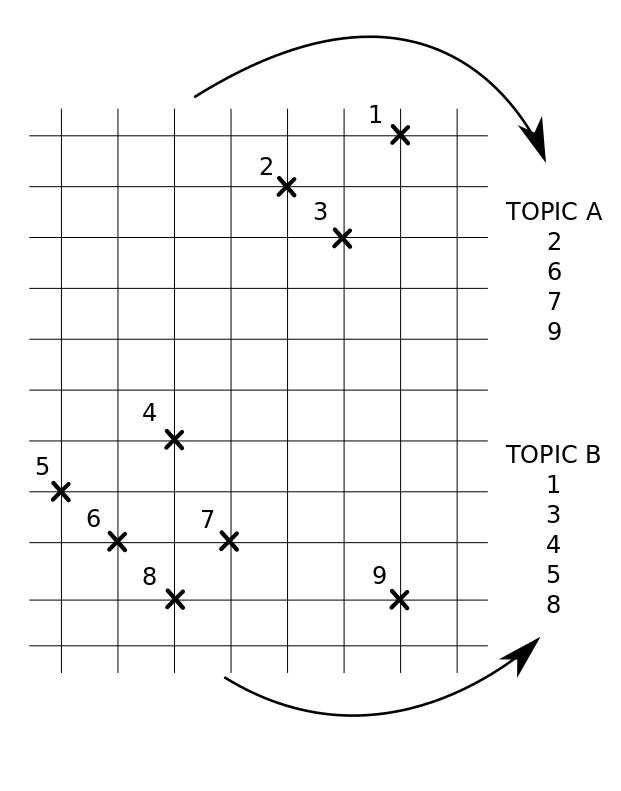
\includegraphics[width=\textwidth]{Pictures/BOW.png}
\caption{The Bag-of-words model with topic assignment.}
\label{fig:FSBOW}
\end{minipage}
~
\begin{minipage}[b]{0.3\linewidth}
\centering
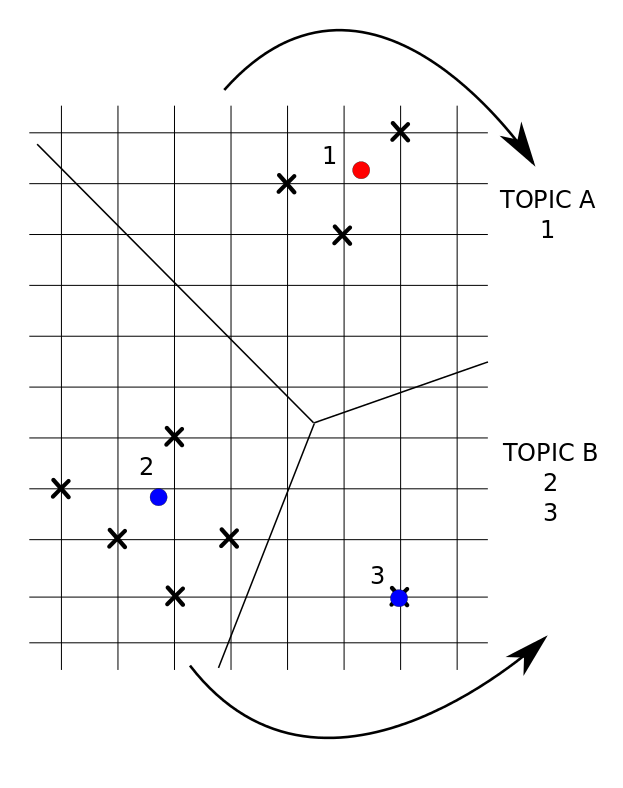
\includegraphics[width=\textwidth]{Pictures/kMeans.png}
\caption{Feature space with k-means and topic assignment.}
\label{fig:FSk-means}
\end{minipage}
~
\begin{minipage}[b]{0.3\textwidth}
\centering
\def\svgwidth{140pt}
\input{Pictures/GMM.pdf_tex}
\caption{Gaussian Mixture Model with LDA}
\label{fig:GMM+LDA}
\end{minipage}
\caption{The two different topics are marked with red and blue.}
\end{figure}

To make sure that similar observations will be grouped together and will appear in the same topic, we can apply the k-means algorithm to find clusters in the data. The id's of the centroids of the clusters then function as 'words' and can be used in the same way as Bag-of-words model, but then with reduced dictionary size. So if we apply LDA to the clustered data some clusters may fall into the same topic. This is shown in figure ~\ref{fig:FSk-means}.\\
The outcome of the LDA model does strongly depend on the outcome of the apriori used cluster algorithm. The clusters that are found with k-means are maybe not a good representation of the data. All clusters may have the same amount of influence on the LDA model, which might not be the correct way to describe the data. The Gaussian Mixture model might give a better description of the clusters. Combining the part of clustering directly into the topic model will avoid the apriori clustering and the clusters are then formed due to the topics, which will give a better globalization of the data. In figure \ref{fig:GMM+LDA} we show how the combination of the part of clustering into the Topic Model might improve the Gaussian Mixture Model.\\
According to the feature representation, which in our case is a discrete derivation of the sensor data, a Poison distribution might be a good choice to model the topic distributions. The Poisson distribution can be used instead of the Gaussian distribution.



% 
% Let us say we have a two dimensional feature space. For example we only have two sensors in our data, than every dimension will refer to one of the sensors. A representation of this model is shown in figure bla (a). A cross marks an observation and is seen as a new 'word' in the bag-of-word method. We can use this data with the LDA model. The problem only with this approach is that similar observations are not group together and it might be possible that a similar observations are not grouped together in the same topic when we apply the LDA model.

% 
% 
% If we cluster the observations on forehand with a the k-means algorithm we can reduce the size of the dictionary (which contains all unique observations) and use again the LDA method to find the topics. The problem here is that there is a hard separation line between the clusters as is shown in figure bla (b).
% 
% So we invented a third method which is a kind of gaussian mixture model included into the LDA topic model. So instead of cluster the model with priors from the data itself we relate the priors directly to the topis and combing the part of clustering and the deriving the topics in one algorithm. In this way clusters are grouped together directly if they belong to the same topic, as is shown in figure bla (c).
% 
% 
% 

% 
% 
% In the next two sections we describe the two different ways how we use the topic models with our data. First we describe the combination of k-means clustering and the basic LDA model as it is described in [Blei]. And after that we describe our new approach that combines the clustering and topic modelling in one algorithm. In this algorithm we step away from the bag-of-words model representation of the data.
%  Nog toevoegen dat we twee manieren gaan gebruiken(LDAbasic and LDAext)
% %%TOT HIER!
% 
% 

%   \subsubsection{K-means}
%  In the previous section we addressed the problem of a wide variance of observations. With a bag-of-words model, as it is used in the LDA approach, similar looking words/observations are not likely to be put in the same topic. All observations, that are not exactly the same, are independent from each other and may not lead to the same topic. Because of the low amount of training data it is not very likely that the same observation will be seen often enough to learn topics from the data properly.
% That is why we need to reduce the amount of unique observations and group similar observations together. In terms of document classification, we could say that we need to reduce the size of the dictionary.


% In a first-approach we use k-means clustering to reduce the size of the dictionary, which is the set of all observations that can be found in the data.
% We do not use the time dimension for the clustering part, because this would compromise our data so that clusters are not detected properly. We use the euclidean distance to determine the best mean.
% 
% maybe preprocess the data with coarse grain time dimension
% 
% size of the dictionary
% is it the case that with a lot of data simialar looking words will be put in the same topic? Or will it just be a different topic?
% 
% 
% 
% In our data the size of the dictionary, which contains all unique observations in the whole corpus is relative large with respect to the size of the data that we have. There are a lot of different observations that are similar to each other, but differ only in one value of the 6 dimensions. So for example the observation $o_1=\{1 ,2 ,5 ,3,14\}$ is similar to the observation $o_2=\{2 ,2 ,5 ,3,14\}$. The only difference of sensor activities is in the first field. In the LDA model these two observations/words will be seen as two different dimensions and the similarities are not captured. In fact a lot of words will only be seen once in the whole corpus and finding good parameters is not possible.
%  So we need to find a way to capture similar observations to build a proper topic model. A simple way is to cluster all observations together and then use the EM-algorithm to estimate the parameters of the  LDA model.
%  For the clustering part we used the k-means algorithm. We reduced the size of the dictionary to 20. After that we use the EM-algorithm as described above.
%  In the clustering we leave out the time dimension because this is fucking up the clusters
 
%   \subsubsection{Latent Dirichlet Allocation with clustered Data}
% The generative model 'Latent Dirichlet Allocation' [Blei] is a way to describe a topic model. In this model it is assumed that a Corpus can be generated from a distribution of topics, where every topic can be represented with a distribution of words. In our case the documents are days and the words are observations $o_n$. In the previous section we described how we reduced the size of the dictionary $V$.
% The generative process that would create the data will look like this:
% 
% For every day that will be generated:
% \begin{enumerate}
%  \item Set the amount of observations in every document to size N (for every day the same amount).
%  \item Choose a topic distribution $\theta \sim Dir(\alpha)$ for the day.
%  \item For each of the N observations $o_n$:
%  
%  \begin{enumerate}
%   \item Choose a topic $z_n \sim Multinomial(\theta)$.
%   \item Choose a set of observations $o_n$ from the set of all observations $V$ from $p(o_n |z_n;\beta)$, a multinomial probability conditioned on the topic $z_n$. Where $\beta$ is the distribution over observations given a topic.
%  \end{enumerate}
% 
% \end{enumerate}
% %!!!Describe the model variables!!!!!
% 
% With the assumption that the data that we got from the sensor system has the same structure than the data created with the generative process we can find the model parameters $\alpha$ and $\beta$ for LDA with the EM-algorithme described in \cite{blei2003latent}.

\section{LDA-Gaussian Model}
In this section we explain how the part of clustering is combined within the LDA model itself. Instead of the k-means clusters we use a Gaussian distribution to model every dimension within the features.


\subsection{Motivation and Assumptions of the Model}
 
Using the cluster algorithm k-mean in advance has some disadvantages. First of all we need to choose the number of clusters. This is not always that easy and then it is still not assured that the best clusters are found. Every cluster also has a hard separation line, which does not give any degradation if a value is far away from the mean of the cluster. There is no quality measurement of the clusters given. So every cluster is equally probable to occur in the topic model, which is not always desirable.

With a Gaussian Mixture Model we might be able to distinguish between more or less important clusters. But we might want to let the topic model decide which topics have more influence and which have not, according to the data.\\
That is why we combined the clustering part and the topic estimation into one step. Instead of a multinomial distribution over all observations that occur in the 'Dictionary', we model a Gaussian distribution over every dimension of the observations. In this way similar observation can be captured in the model itself and are not generalized in one cluster beforehand.\\
The difference is that instead of a large, fixed set of unique observations (Dictionary), with a multinomial distribution, we take a Gaussian distribution over every dimension of the observations. In this way smoothing is not necessary, because unseen observations will be handled properly.
In the next sections we describe the model in more detail. We first give an overview of the generative process. Then we explain the variational inference that is necessary to make the parameter estimation possible. And finally explain the EM-algorithm that determines the parameters.

% Every topic will have its own distribution over the dimensions. A
% topic can be described as shown in figure %\ref{fig:topic}.
% In this figure an example of a topic description is shown
% \begin{figure}
%  \includegraphics[\width=\textwidth]{Pictures\topics.png}
%  \caption{An awesome topic}
%  \label{fig:topic}
% \end{figure}

  \subsection{Model Description}
  
  Our model assumes that every day in a dataset can be represented as random mixtures of latent topics, where every topic can be described as a distribution over observations. We assume the following generative procss for every day $m$ in the data set $C$:
\begin{enumerate}
 \item The amount of observations on a day $m$ is fixed with size $N$ (for every day the same size).
 \item A day has a distribution over the topics given with $\theta \sim Dir(\alpha)$.
 \item For each of the N observations on a day $o_n$:
 
 \begin{enumerate}
  \item Estimate the topic $z_n \sim Multinomial(\theta)$.
  \item An observation $o_n$ is gained from $p(o_n |z_n,\boldsymbol\mu,\boldsymbol\sigma)$,  which is a probability that can be drawn from a set of Gaussian distributions. This probability is conditioned on the topic $z_n$ and the Gaussian Parameters $\vec{\mu_i}$ and $\vec{\sigma_i}$ of length $d$ that belong to the estimated topic $i$.
 \end{enumerate}

\end{enumerate}
  
In this model the amount of topics $k$ is assumed to be known and fixed and with it the size of the topic variable $z$.
The probability for the observations is parametrized with two matrices $\boldsymbol\mu$ and $\boldsymbol\sigma$, both of size $D\times k$, where $D$ is the amount of dimensions in an observation and $k$ the amount of topics. They present the mean and standard deviation respectively and for every topic $i$ and every dimension $d$ there is a set of parameters, which describes a Gaussian distribution. Every value of a dimension for an observation $o_{ndi}$ can then be drawn from a Gaussian Distribution $\mathcal{N}(\mu_{di},\sigma_{di})$.
The size of the dimension $D$ is assumed to be fixed and a more extensive description of the representation of the observations is given in section \ref{sec:features}. $\alpha$ represents the Dirichlet parameter and is vector of length $k$.

In figure \ref{fig:modelExt} the graphical representation of the model is shown. It differs from the basic LDA model (figure \ref{fig:modelBasic}) in the description of the topic distribution $\beta$, which is here replaced with $\mu$ and $\sigma$.

\begin{figure}[h!]
\centering
\def\svgwidth{0.8\textwidth}
\input{Pictures/ModelExt.pdf_tex}
\caption{Graphical representation of the LDA-Gaussian model}
\label{fig:modelExt}
\end{figure}




  
Assuming that the generative process described above can describe the available data properly, we now want to find the parameters so that the model best describes our data. We want in fact maximize the probability for the dataset $C$ given the model with respect to the parameters $\alpha$, $\mu$ and $\sigma$. This probability looks like this
\begin{equation}
p(C|\alpha,\mu,\sigma) = \prod_{m=1}^M p(m|\alpha,\mu,\sigma)
\end{equation}
where $M$ is the amount of days within the dataset and the probability for a day $m$ given the three parameters, which is the marginal distribution over a day, is
\begin{equation} 
p(m|\alpha,\mu,\sigma) = \int p(\theta|\alpha)  \left( \prod_{n=1}^N \sum_{z_n} p(z_n|\theta) p(w_n|z_n, \mu,\sigma)  \right) d\theta
\end{equation}
This distribution is gained by integrating the joint distribution \ref{eq:Joint} by $\theta$.
\begin{equation} \label{eq:Joint}
 p(\theta,\textbf{z},\textbf{w}|\alpha,\mu,\sigma) = p(\theta|\alpha) \prod_{n=1}^N p(z_n|\theta) p(w_n|z_n,\mu,\sigma)
\end{equation}
In the next section we describe how we can find the optimal parameters for the model given a data set.


  
\subsection{Variational Inference}
 
The marginal distribution, which is given in the previous section, can be written in terms of the parameter $\alpha$, $\mu$ and $\sigma$ as
  \begin{equation}
   p(m|\alpha,\mu,\sigma) = \frac{\Gamma (\sum_i \alpha_i)}{\prod_i \Gamma(\alpha_i)} \int \left( \prod_{i=1}^k \theta_i^{\alpha_i-1} \right)
   \left( \prod_{n=1}^N \sum_{i=1}^k \prod_{d=1}^D \theta_i \mathcal{N}(o_{nd},\mu_{id},\sigma_{id} ) \right)
  \end{equation}
Due to the coupling between $\theta$ and the Gaussian parameters $\mu$ and $\sigma$ this probability is intractable to compute.	




That is why we use a convexity-based variational algorithm to approximate the log-likelihood of a given dataset. 
An approximation of the model is given with 
  \begin{equation}
   q(\theta,z|\gamma,\phi) = q(\theta|\gamma) \prod_{n=1}^N q(z_n|\phi_n).
  \end{equation}
In this model $\gamma$ represents the Dirichlet parameter and $\phi$ are the multinominal parameter which can be viewed as the probabilty $p(z_i|o_n)$ and is given as a $k \times N$-matrix for every day $m$. The graphical representation of the model is shown in figure \ref{fig:ModelApprox}.
  
 
\begin{figure}[h!]
\centering
\def\svgwidth{0.4\textwidth}
\input{Pictures/ModelApprox.pdf_tex}
\caption{Approximation of the model.}
\label{fig:ModelApprox}
\end{figure}
 
  
  
  
  Given the variational distribution for aproximate model we can estimate the lower bound of the log-likelihood with the Jensen inequality as
  \begin{equation}
   \begin{split}
    L(\gamma;\phi;\alpha;\mu;\sigma) =& E_q[\log p(\theta|\alpha)] + E_q[\log p(\textbf{z}|\theta)] + E_q[\log p(\textbf{w}|\textbf{z},\mu,\sigma)] \\
   & -E_q[\log p(\theta)] - E_q[\log q(\textbf{z})]
   \end{split}
  \end{equation}

In terms of the model parameters and the variational parameters this becomes
\begin{equation}
  \begin{split}
 L(\gamma;\phi;\alpha;\mu;\sigma) =& \log \Gamma (\sum_{j=1}^k \alpha_j) - \sum_{i=1}^k \log \Gamma(\alpha_i) + \sum_{i=1}^k (\alpha_i-1)(\Psi(\gamma_i)-\Psi(\sum_{j=1}^k \gamma_j)) \\
 & + \sum_{n=1}^N \sum_{i=1}^k \phi_{ni} (\Psi(\gamma_i)-\Psi(\sum_{j=1}^k \gamma_i)) \\
  & + \sum_{n=1}^N \sum_{i=1}^k \sum_{d=1}^D \phi_{ni} \log( \mathcal{N}(o_{nd};\mu_{id},\sigma_{id})) \\
  & - \log \Gamma (\sum_{j=1}^k \gamma_j) + \sum_{i=1}^k \log \Gamma (\gamma_i) - \sum_{i=1}^k (\gamma_i -1)(\Psi(\gamma_i)-\Psi(\sum_{j=1}^k \gamma_j)) \\
 & - \sum_{n=1}^N \sum_{i=1}^k \phi_{ni} \log \phi_{ni}
  \end{split}
  \label{eq:likeli}
\end{equation}
With an EM process we are then able to maximize this lower bound on the log-likelihood. The two steps are:
  \begin{enumerate}
   \item \textbf{E-step:} For each day $m$, optimize the variational parameters $\{ \gamma_{m}*,\phi_{m}* \}$
   \item \textbf{M-step:} Maximize the resulting lower bound on the log-likelihood with respect to the model parameters $\alpha$, $\mu$ and $\sigma$.
  \end{enumerate}
  
  We now give a more detailed description on both of these steps.
  
  \paragraph{E-step}
In the e-step of the algorithm the variational parameters $\phi$ and $\gamma$ are optimized. To get the update function for $\phi$ we get all terms of the lower bound of the loglikelihood in equation (\ref{eq:likeli}) that contains the variable $\phi$. 
Take $y_i=\sum_{d=1}^D \mathcal{N}(o_{nd};\mu_{id},\sigma_{id})$
We add the constraint $\sum_{i=1}^k \phi_{ni}=1 $ to the formula and get
\begin{equation}
 L_{[\phi_{ni}]} = \phi_{ni}(\Psi(\gamma_i)-\Psi(\sum_{j=1}^k \gamma_j)) + \phi_{ni} \log(y_i) + \lambda_n(\sum_{j=1}^k \phi_{ni} -1)
\end{equation}
From this equation we take the derivative of the formula and set it to zero. This leads to the first update function
\begin{equation}
 \phi_{ni} \propto \log(y_i) \exp(\Psi(\gamma_i) - \Psi(\sum_{j=1}^k \gamma_j))
\end{equation}\\
For $\gamma$  we also take all terms of equation \ref{eq:likeli} that contain this variable and set the derivate to zero. This leads to the second update equation
\begin{equation}
 \gamma_i = \alpha_i + \sum_{n=1}^N \phi_{ni}
\end{equation}

  %Nu nog de algorithme geven

  \paragraph{M-Step}
  
In the m-step the parameters of the Gaussian distribution $\mu$ and $\sigma$ are estimated with the weighted arithmetic mean calculated over all observation in a dataset given the parameter $\phi$, which is gained in the previously e-step. This leads to the update formulas
\begin{equation}
 \mu_{di} = \frac{\sum_{m=1}^M \sum_{n=1}^N o_{dn} \phi_{ni} }{\sum_{m=1}^M \sum_{n=1}^N  \phi_{ni}}
\end{equation}
and
\begin{equation}
 \sigma_{di} = \sqrt{\frac{\sum_{m=1}^M \sum_{n=1}^N o_{dn}^2 \phi_{ni} }{\sum_{m=1}^M \sum_{n=1}^N  \phi_{ni}} - \mu_{di}^2}
\end{equation}\\
To calculate the parameter $\alpha$ we again take all terms of the likelihood that contains the variable $\alpha$. The derivative in the Hessian form is
\begin{equation}
 \frac{\partial L}{\partial \alpha_i\alpha_j} =  m(i,j) M \Psi'(\alpha_i) - \Psi'(\sum_{j=1}^k \alpha_j)
\end{equation}
On this equation we can use the Newton-Rhapson method to calculate the optimal $\alpha$.

\section{LDA-Poisson Model}


If the features are described in a discrete way, which means that every dimension has an integer value, the Poisson distributions is a better choice to describe the data. In figure \ref{fig:LDAPoisson} the graphical representation of LDA-Poisson model is shown. 

\begin{figure}[h!]
\centering
\def\svgwidth{0.8\textwidth}
\input{Pictures/ModelPois.pdf_tex}
\caption{Graphical representation of the LDA-Poisson model.}
\label{fig:LDAPoisson}
\end{figure}

The variational Inference and the EM-procedure will be the same as described before, except for the Gaussian distribution that is exchanged with the Poisson distribution. The parameter $lambda$ which describes the Poisson distribution is calculated in the M-step with
\begin{equation}
 \lambda_{di} = \frac{\sum_{m=1}^M \sum_{n=1}^N o_{dn} \phi_{ni} }{\sum_{m=1}^M \sum_{n=1}^N  \phi_{ni}}.
\end{equation}



% For a reason 
% the reason is that lda captures priors for the days, that are given with the 
% which is still not is clear for me, we combine the clustering and determining of the topics in one algorithm.
% Preprocessing the data with k-means may not capture the topic distributions probably. The time dimension is not taken into account in the clustering part. So we want to avoid the preprocessing the data with k-means and add the the clustering part directly in the model.
% So first we describe how the model will change with respect to the LDA model descriibed above (or maybe: ... how extension of the LDA model looks like) and we also describe how the parameters are determined with the EM algorithm.
% 
% 
% So what is different? Maybe do not ask this question but just explain how the model looks like.
% 
% The main change of the model is that it is also captures similar observation in one topic.
%  So instead of describing a topic only with one discrete value in one dimension, we model every dimension in the observation with a Gaussian distribution. So every dimension given a topic needs to be defined with a mean and a standard deviation. The dimension might depend from each other
% 
% 
%   This is done in the following way:
% Instead of storing the probability for a observation given a topic, which is done in the matrix $\beta$, we assume that every dimension of the observations is normal distributed given a topic. So we store the mean and variance for every dimension given a topic in two matrices of size $d \times k$ where $d$ is the dimension of the observations and $k$ the amount of clusters. For now we assume that the dimensions of the observations are uncorrelated. The EM-algorithm is adjusted to calculate the $\beta$- matrix properly.
% 
% - The combination of the k-means clustering and the LDA model might not capture the topics correctly. The k-means clustering gives a hard boundaries on the words, which is also a drawback from the sequential combination of clustering and topic estiamtion. Therefore we want to comine these two step in one.


\clearemptydoublepage

\chapter{Experiments}\label{chapter:experiments}
In this chapter the experiments and the results are presented. In the section of the qualitative results visualizations of the topics are given for different models. It is shown that the topics are meaningful and that semantic descriptions can be given to some of these topics.
In the section of the quantitative results the two developed models are compared with each other and the performance of the model for different number of topics and different number of time-slices are shown.

\section{Qualitative Results}
\subsection{Comparison of the different models}
%wat wordt er in deze sectie getoond?
In this section four different models are compared with each other. The first two models are the LDA model with a Bag-of-word representation, where the dictionary one the one hand is pre-clustered with the k-means algorithm(LDA with BOW + k-means, figure \ref{fig:BOWtopics} a)) and on the other hand not clustered at all (LDA with BOW, figure \ref{fig:BOWtopics} b)). The third and fourth model are LDA-Gaussian and LDA-Poisson (figure \ref{fig:Gaus96} and \ref{fig:Pois96}).\\

% wat is in de plaatjes te zien?
In the following figures the number of time-slices on a day is $N=96$. The time dimension is a coarse-grain representation, which means that there are five different values for the time. The number of topics that are initialized are $k=5$. Figures \ref{fig:BOWtopics} a) + b), \ref{fig:Gaus96} a) and \ref{fig:Pois96} a) are a representation of the topic distribution on different days. There are in total 50 days represented on the y-axis in each figure. On the x-axis the time-slices are shown. The different colors represent the different topics that are assigned to the time-slices.\\

\begin{figure}
 \centering
 \begin{tabular}{c c}
  \centering
  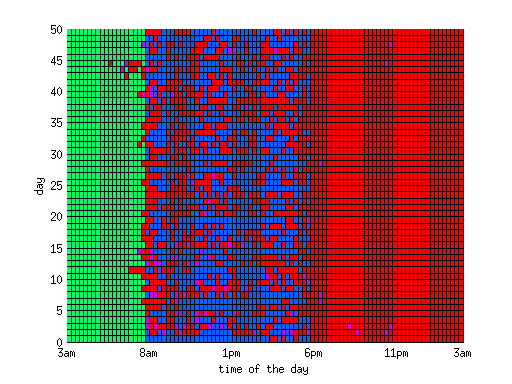
\includegraphics[width=0.45\textwidth]{Pictures/DayTopicsTs96k5Clus.png}
  &
  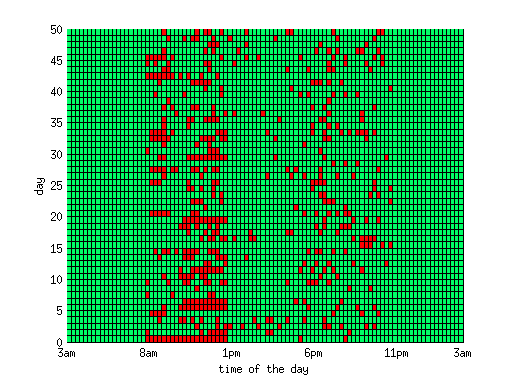
\includegraphics[width=0.45\textwidth]{Pictures/DayTopicsTs96k5bow.png}\\
  a) & b)
 \end{tabular}
 \caption{a) LDA model applied to clustered data. b) LDA applied to data that is not clustered.}
 \label{fig:BOWtopics}
\end{figure}

\pagebreak
 
The LDA model with a BOW-representation is still able to find different topics in the data, although the BOW representation without the clustering only distinguish between two topics (see figure \ref{fig:BOWtopics} b)). If the data is clustered on forehand LDA is able to find four different topics in the data (see figure \ref{fig:BOWtopics} a)). The number of clusters for the k-means algorithms is set to $V=6$. This was the best value to find the most topics in the data. Before the data was clustered, all dimensions where normalized.\\

\begin{figure}
 \centering
 \begin{tabular}{c c}
  \centering
  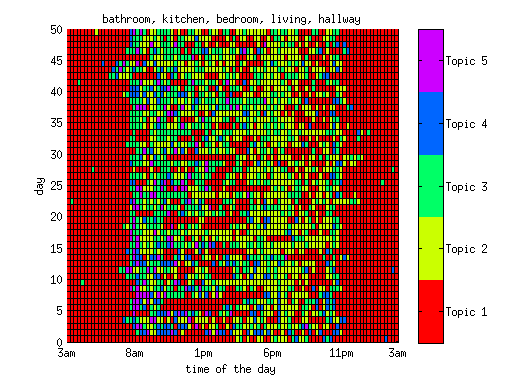
\includegraphics[width=0.45\textwidth]{Pictures/TopDayHN3TS96k5Gaus.png}
  &
  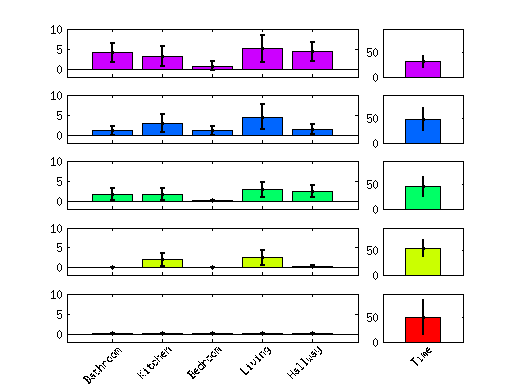
\includegraphics[width=0.45\textwidth]{Pictures/TopVisuHN3TS96k5Gaus.png}\\
    a) & b)
 \end{tabular}
 \caption{Topic distribution per day and the Topic visualization for LDA-Gaussian}
 \label{fig:Gaus96}
\end{figure}  

Figure \ref{fig:Gaus96} shows the outcome of the LDA-Gaussian model. In the figure on the right-hand side (\ref{fig:Gaus96} b) ) the 6 dimensions of the observations are shown on the x-axis. Every topic is marked with a different color and corresponds to the topics in the left image. On the y-axis the mean value $\mu$ of every Gaussian distribution in every dimension is indicated with the height of the bar-chart. The vertical black line represents the standard deviation $\sigma$ of every distribution. The red topic (topic 1) contains a high $\sigma$-value for the time-dimension and captures all time-slice where the value is zero for the sensor values. LDA-Gaussian is able to find more notable topics and leads to more meaningful results than it can found with LDA for a BOW representation. For example the daily structure of a person can be distinguished more easily than it can be done in figure \ref{fig:BOWtopics} a) or b).\\

\pagebreak
\begin{figure}
 \centering
 \begin{tabular}{c c}
  \centering
  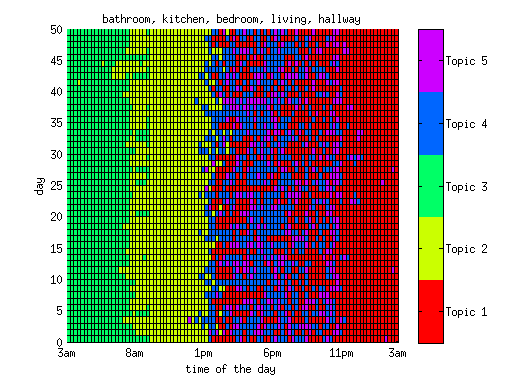
\includegraphics[width=0.45\textwidth]{Pictures/TopDayHN3TS96k5Pois.png}
  &
  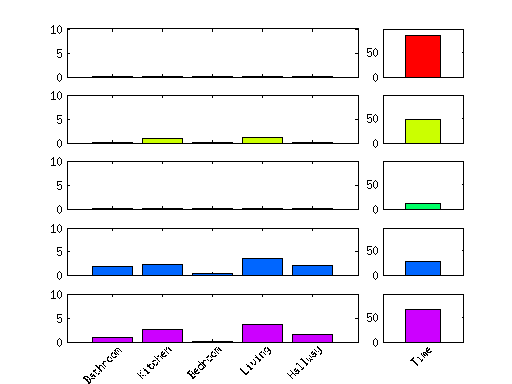
\includegraphics[width=0.45\textwidth]{Pictures/TopVisuHN3TS96k5Pois.png}\\
    a) & b)
 \end{tabular}
 \caption{Topic distribution per day and the Topic visualization for LDA-Poisson}
 \label{fig:Pois96}
\end{figure}  


In figure \ref{fig:Pois96} the outcome of the LDA-Poisson model is shown. The topics that are found are again shown on the right-hand side (\ref{fig:Pois96} b) ). The height of the bars represent the $\lambda$-value of the Poisson-distributions.
In the figure \ref{fig:Pois96} a) five different topics are found. These topics depend however a lot on the time. This is caused by the fact that the Poisson distribution is not a good way to model the time dimension, because small values will have a higher probability in this distribution. Nevertheless LDA-Poisson still performs better, than LDA on the BOW representation.



\subsection{Semantic topic description}
In the following figures the topic distribution for different houses are shown. A semantic description of some topics is given to illustrate the usefulness of the models. The number of time-slices is set to $N=48$. In every figure 50 days are shown. In the left images a) the topic distribution of the days are shown and in the left images b) the topic description for every dimension is given with respectively the same color. For more results see the appendix \ref{chapter:appendix_1}.\\

In figure \ref{fig:HN1Gaus20fine} the outcome for the LDA-Gaussian model is shown. The time dimension has a fine grain representation. The model is initialized with $k=20$ topics and the 10 most important topics are visualized with a different color, the remaining topics have the color gray in the left image. The first topic (red) is an easy topic to find. In all time-slices that are marked with red no activations of the sensors are captured. The time dimension has a big standard deviation, because this topic can occur all day long. In figure \ref{fig:HN1Pois20fine}, which is outcome of the LDA-Poisson model with same values, thi topic is divided in two different topics (red and orange). These topics only distinguish between the time value. Comparing the two outcomes (figure \ref{fig:HN1Gaus20fine)} and \ref{fig:HN1Pois20fine}) one can see that topics of the LDA-Gaussian model are much easier to interpret. For example the ninth topic (purple) can be seen as the topic `preparing for bed'. This topic cannot be found in the outcome of the LDA-Poisson model. The topic `going to toilet', which is the third topic (yellow) in the LDA-Gaussian model is also not shown in the outcome of the LDA-Poisson model.\\

In figure \ref{fig:HN5Gaus20fine} the `going to toilet' is also present. This figure shows the outcome for House number 5 with the LDA-Gaussian model. Here two topics (purple and pink) can be found, which indicates the `morning preparations'. Every week the person seems to leaving the house in the afternoon and comes back around 11 pm. Comparing house number 1 and 5 with each other one can see that the person that is living in house number 5 goes to bed a little bit earlier than the person living in house number 1.\\

More topics can be appointed and for some person it appears easier than for other person. The main point however is that indeed a daily or even weekly structure can be found with distributions of the topics during a day. 

\begin{figure}[h!]
 \centering
 \begin{tabular}{c c}
  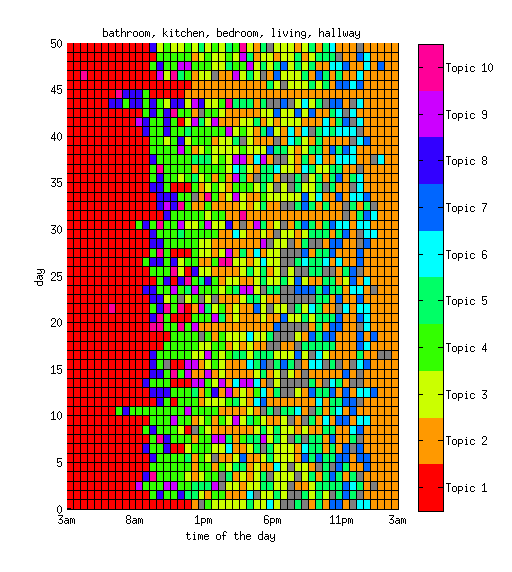
\includegraphics[width=0.45\textwidth]{Pictures/Pois/fine/DayHN1TS48k20fine.png}
  &
  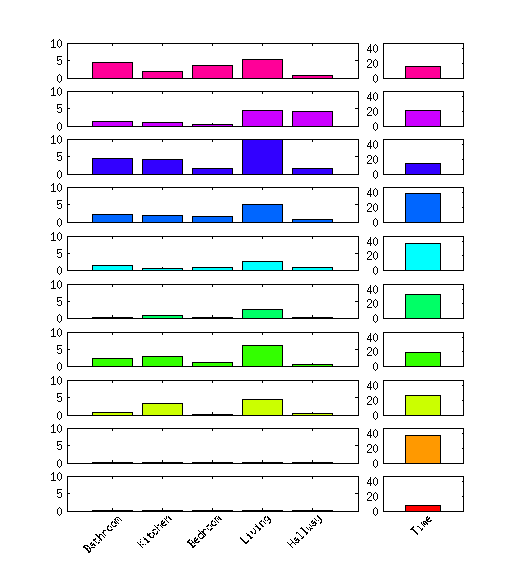
\includegraphics[width=0.45\textwidth]{Pictures/Pois/fine/TopHN1TS48k20fine.png}\\
  a) & b)
 \end{tabular}
  \caption{House number 1, 20 topics, fine grain time, LDA-Poisson}
  \label{fig:HN1Pois20fine}
\end{figure}

\begin{figure}
 \centering
 \begin{tabular}{c c}
  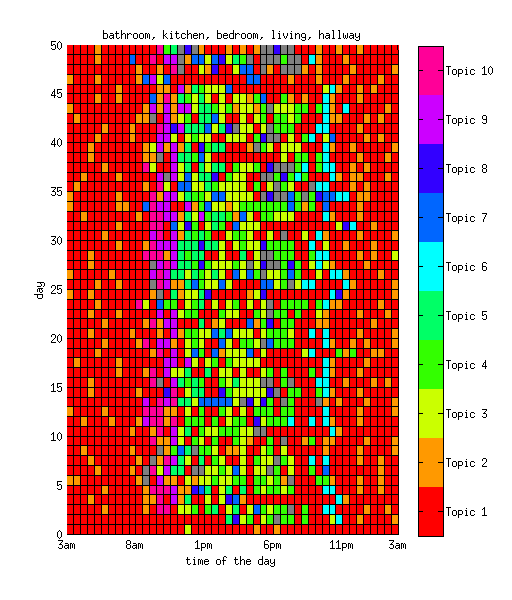
\includegraphics[width=0.45\textwidth]{Pictures/Gaus/fine/DayHN5TS48k20fine.png}
  &
  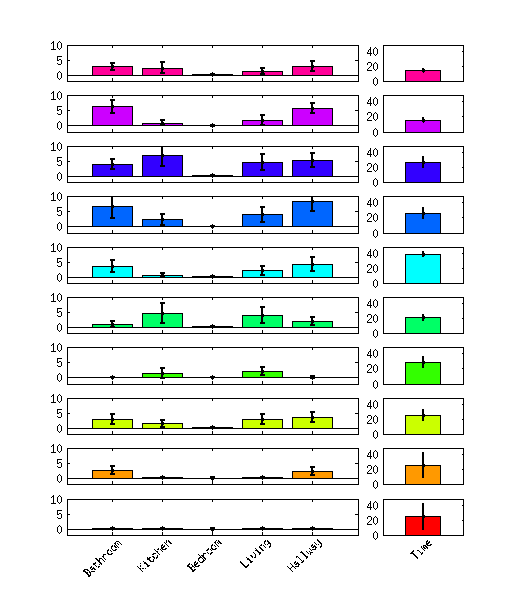
\includegraphics[width=0.45\textwidth]{Pictures/Gaus/fine/TopHN5TS48k20fine.png}\\
  a) & b)
 \end{tabular}
  \caption{House number 5, 20 topics, fine grain time, LDA-Gaussian}
  \label{fig:HN5Gaus20fine}
\end{figure}

\begin{figure}
 \centering
 \begin{tabular}{c c}
  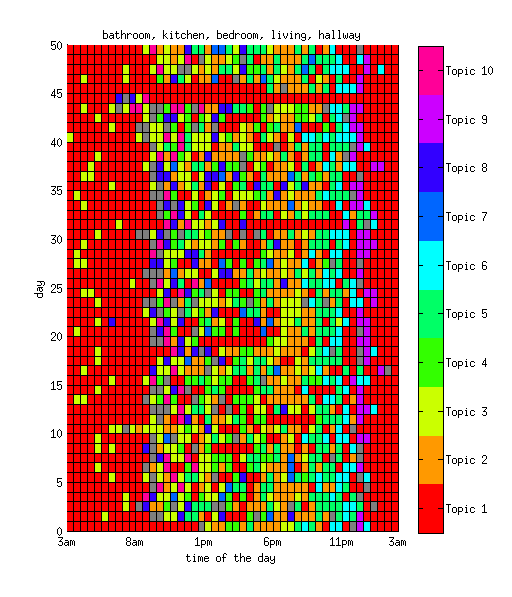
\includegraphics[width=0.45\textwidth]{Pictures/Gaus/fine/DayHN1TS48k20fine.png}
  &
  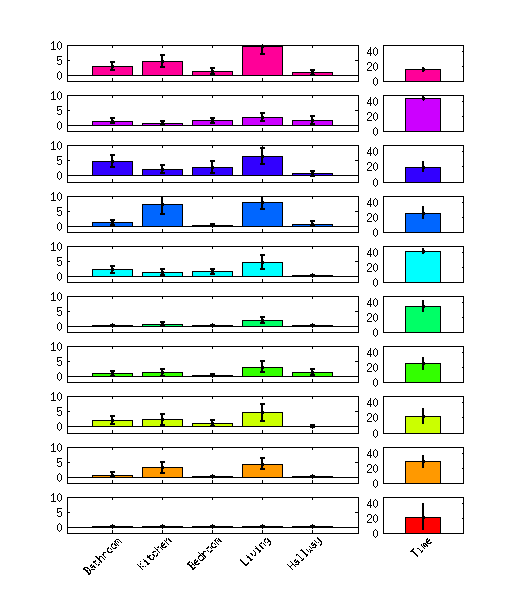
\includegraphics[width=0.45\textwidth]{Pictures/Gaus/fine/TopHN1TS48k20fine.png}\\
  a) & b)
 \end{tabular}
  \caption{House number 1, 20 topics, fine grain time, LDA-Gaussian}
  \label{fig:HN1Gaus20fine}
\end{figure}

\pagebreak

\subsection{Quantitative Results}
The log-likelihood indicates on how well the model with the estimated parameters fits the data. This can easily overfit and new data can not easily modeled with the found parameters. Therefor it is necessary to also find a high log-likelihood on a hold-out-set. The perplexity gives a good indication on how and can be calculated with
\begin{equation}
 perplexity(D_{HOS}) = exp \left\{ - \frac{\sum_{m=1}^M \log p(\textbf{o}_d ) }{M*N} \right\}
\end{equation}

A low perplexity value indicates a good result on the hold-out-set.\\

In the next experiments 10\% percent of the data is used as a hold-out set. The model is trained on the remaining 90\% with different initialization values and the perplexity is calculated on the hold-out-set with the estimated parameters. In the following it is shown what the effect is on different number of topics and different numbers of time-slices. Also the two models LDA-Gaussian and LDA-Poisson are compared with each other.

\paragraph{Different Sets of Data}
In figure \ref{fig:PerplGaus} the perplexity is shown for the 5 different data-sets gained from the 5 houses. Every run is performed ten times and the mean over these runs is taken for different number of topics $k$. Every run is initialized with 5 random days.
The data sets vary in length, but as one can see in the figure, the amount of data is not necessary of influence how well the LDA-Gaussian model can be trained. Some data sets are much more stable than others and this is probably due to the way how regular peoples behavior is.

\begin{figure}[h!]
 \centering
 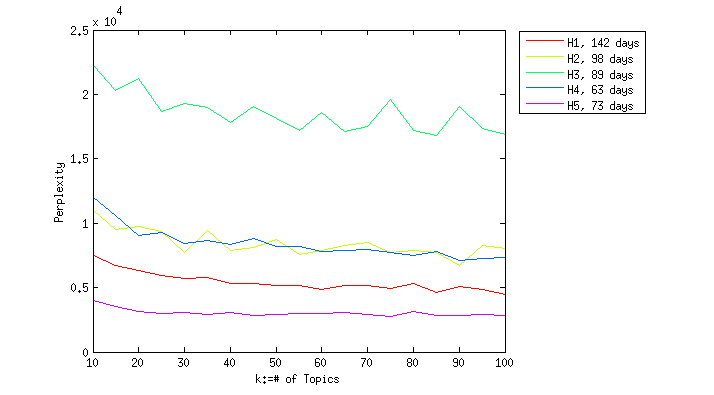
\includegraphics[width=0.7\textwidth]{Pictures/PerplGaus.png}
 \caption{Perplexity for different number of topics for 5 different House}
 \label{fig:PerplGaus}
\end{figure}

\pagebreak
\paragraph{Comparison LDA-Gaussian and LDA-Poisson}
The LDA-Poisson model is not capable to model the time dimension properly. To be able to compare both models directly with each other the time dimension is left out in the following experiments. The perplexity is calculated for the hold-out set with different amount of time-slices and the mean of 10 runs for different number of time-slices is shown in figure \ref{fig:CompareTS}. The perplexity gets better if the number of time-slices increases, but at one point the there will be no improvement. If the length of the time-slices becomes so small that only one activation is captured in an observation, the model perplexity becomes indeed very high, because a topic only contains one value. The topics are then however not very informative.\\

\begin{figure}[h!]
 \centering
  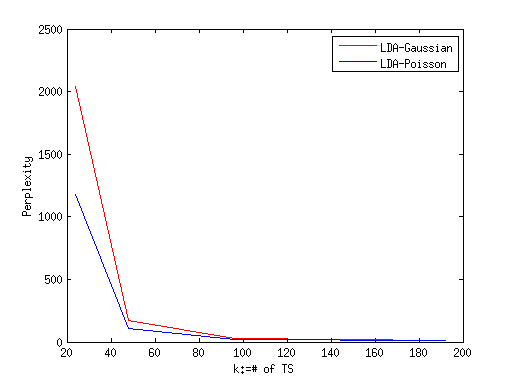
\includegraphics[width=0.7\textwidth]{Pictures/CompareTSgausPois.png}
  \caption{Perplexity for LDA-Gaussian and LDA-Poisson with different amount of time-slices}
  \label{fig:CompareTS}
\end{figure}

In figure \ref{fig:CompareK} the perplexity for both models is shown with different number of topics. The mean of 10 runs is shown and also the standard deviation is indicated with the vertical errorbar in the figure. The standard deviation increases for a higher number of topics, which is reasonable, because more topics increases the chance of more variation. If the number of topic increases the perplexity first decreases and then increases. If the number of topics is to high the model does overfit on the training data and the perplexity indeed becomes worse.\\




 \begin{figure}[h!]
  \centering
  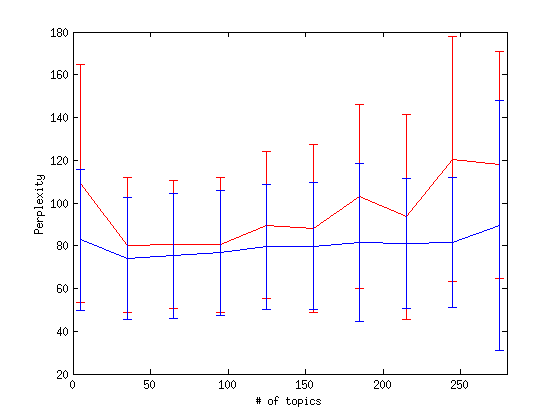
\includegraphics[width=0.7\textwidth]{Pictures/CompareCrossTops.png}
\caption{Perplexity for LDA-Gaussian and LDA-Poisson with different amount of topics}
  \label{fig:CompareK}
 \end{figure}


To creating the figures the data of house number 2 is chosen. For other data sets the outcomes looks similar and are therefore not presented. Both experiments show that the LDA-Poisson model outperforms the LDA-Gaussian model.
 
 
% \paragraph{Different length of time-slices}
% 
% In figure \ref{fig:PerplTS} we give the perplexity for different length of time-slices for the 5 Houses. We take a again the mean over 10 runs. We take for every house the same amount of days to train and test the data. We can see that with more time-slices the perplexity becomes lower for the hold-out set. For house $H2$ and $H4$ the perplexity is much better for a small amount of time-slices. The perplexities for these two houses drop much faster if the amount of time-slices increases.
% 
% \begin{figure}[h!]
%  \centering
%  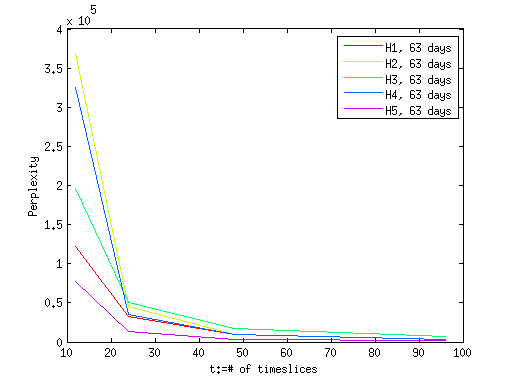
\includegraphics[width = 0.7\textwidth]{Pictures/PerplTS.png}
%  \caption{Perplexity (x-axis) for the hold-out-set for different amount of time-slices (y-axis)}
%  \label{fig:PerplTS}
% \end{figure}


% Wat wil ik nou eigenlijk aantonen en kan ik dat ook aantonen?
% Ik wil aantonen dat het nieuwe model werkt. Ik wil aantonen dat het beter werkt dan normal LDA model. 
% Het is al door meerdere mensen aangetoond dat topic modellen wel van nut zijn om behavior patronen in sensor data te vinden.
% en we kunnen dus aantonen dat onze nieuwe methode OOK werkt, want we kunnen patterns vinden. eg: een dag in de week is de persoon in de middag weg, of 's nachts moet die persoon naar het toilet

% QUALITATIVE EXPERIMENTEN
%Ik wil aantonen dat mijn model werkt en dat je wel zinnige informatie eruit kunt halen. Je kunt een semantische omschrijving van de topics geven.
%We vergelijken de nieuwe method met de BOW/k-means methode we kunnen hier ook aangeven wat de verhoudingen zijn van worden in de data en unique worden die zijn gevonden. Dit geeft ook al aan dat BOW waarschijnlijk niet werkt


%Met de gegeven data en de gekozen feature representation zijn we niet in staat om zinnige informatie uit de BOW model te halen.

% QUANTITATIVE EXPERIMENTEN


% In this section we first give some qualitative results, where the topic distribution on some days are shown. 
% Then we do something else
% Then we compare the BIC's?
% And after that we make a small test according to the feature representation.


%To test the performance of the topic models we set the variables of the features to fixed values.  In the basic LDA model we use a coarse grain value for the time. This means that the sixth dimension can have 5 different values, where the time intervals are $\{ 3am - 8am, 8am - 1pm, 1pm - 18pm, 18pm - 23pm, 23pm - 3am  \}$.

\clearemptydoublepage

\chapter{Conclusions}\label{chapter:conclusions}
Write your conclusions here.

\clearemptydoublepage

%Choose a good bibliography style, plain would do often, but these might be nice too
%\bibliographystyle{these}
\bibliographystyle{plain}
\bibliography{references}

 \clearemptydoublepage
 
 \appendix
 \addcontentsline{toc}{chapter}{Appendix}
 
 \chapter{LDA-Gaussian}
\label{A}
In this part of the appendix the results for all houses are shown for the LDA-Gaussian model. The number of time-slices is $n=48$ and the number of topics is $k=20$. The time dimension has a fine grain representation.

\paragraph{LDA-Gaussian}
Here the outcome of the LDA-Gaussian model is shown.

\begin{figure}[h!]
 \centering
 \begin{tabular}{c c}
  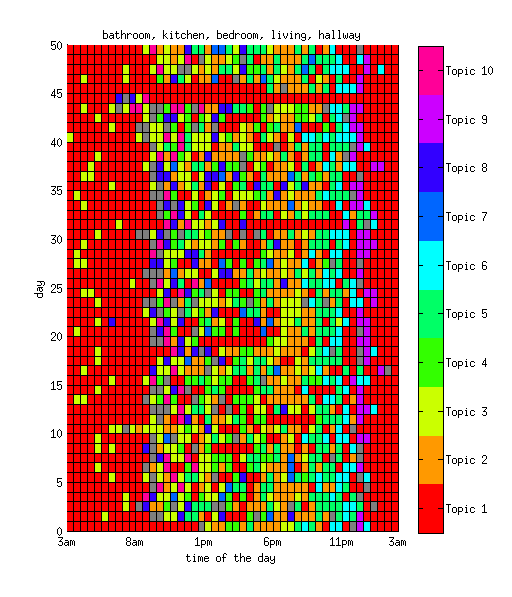
\includegraphics[width=0.45\textwidth]{Pictures/Gaus/fine/DayHN1TS48k20fine.png}
  &
  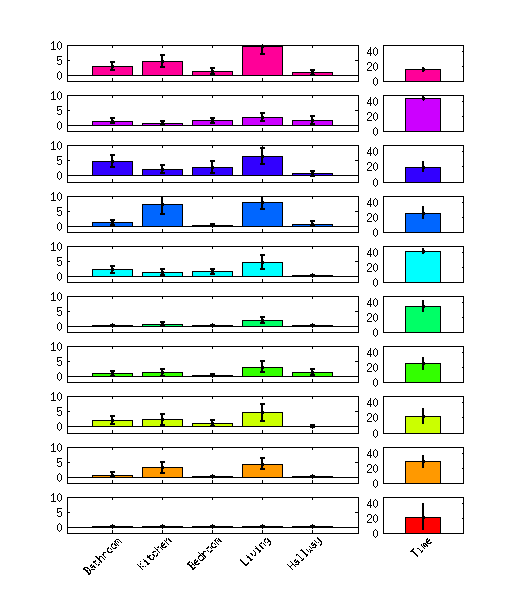
\includegraphics[width=0.45\textwidth]{Pictures/Gaus/fine/TopHN1TS48k20fine.png}\\
  a) & b)
 \end{tabular}
  \caption{House number 1, 20 topics, fine grain time, LDA-Gaussian}
\end{figure}

\begin{figure}[h!]
 \centering
 \begin{tabular}{c c}
  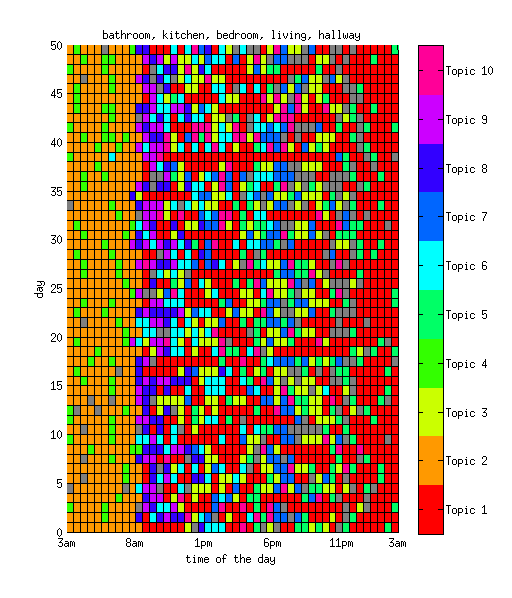
\includegraphics[width=0.45\textwidth]{Pictures/Gaus/fine/DayHN2TS48k20fine.png}
  &
  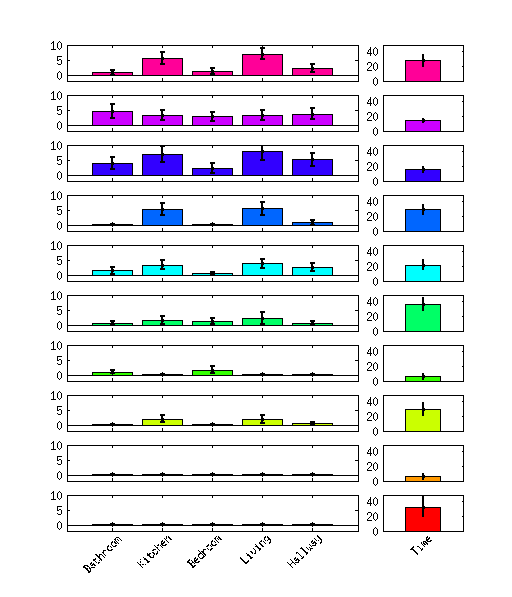
\includegraphics[width=0.45\textwidth]{Pictures/Gaus/fine/TopHN2TS48k20fine.png}\\
  a) & b)
 \end{tabular}
  \caption{House number 2, 20 topics, fine grain time, LDA-Gaussian}
\end{figure}

\begin{figure}[h!]
 \centering
 \begin{tabular}{c c}
  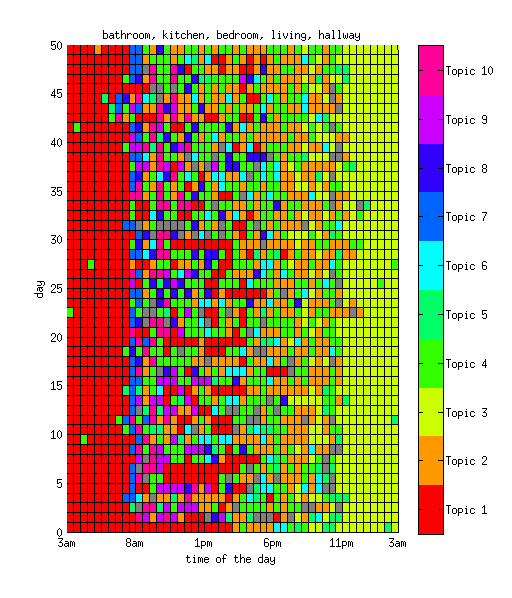
\includegraphics[width=0.45\textwidth]{Pictures/Gaus/fine/DayHN3TS48k20fine.png}
  &
  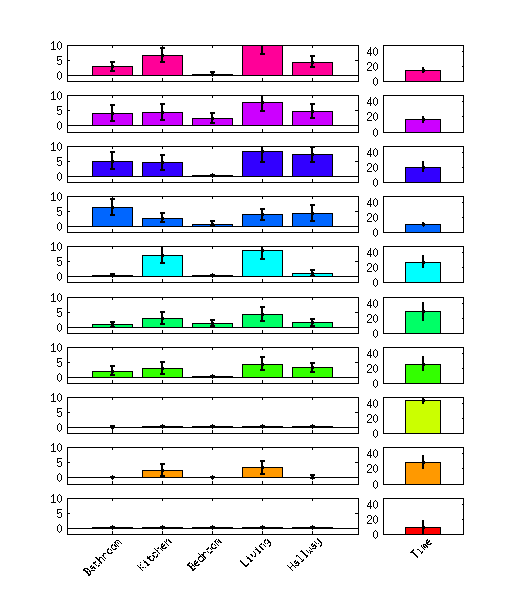
\includegraphics[width=0.45\textwidth]{Pictures/Gaus/fine/TopHN3TS48k20fine.png}\\
  a) & b)
 \end{tabular}
  \caption{House number 3, 20 topics, fine grain time, LDA-Gaussian}
\end{figure}

\begin{figure}[h!]
 \centering
 \begin{tabular}{c c}
  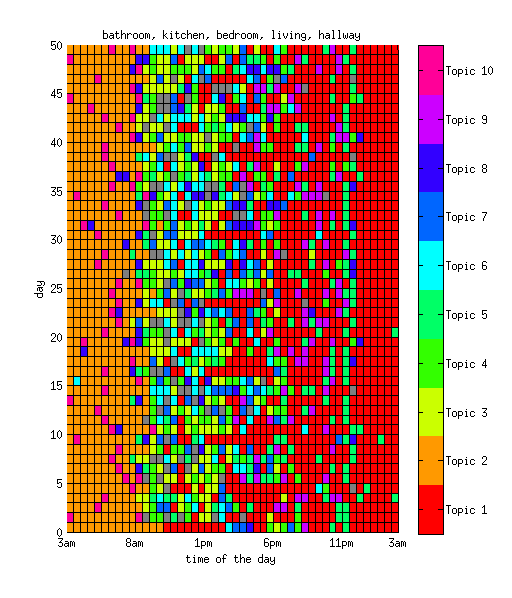
\includegraphics[width=0.45\textwidth]{Pictures/Gaus/fine/DayHN4TS48k20fine.png}
  &
  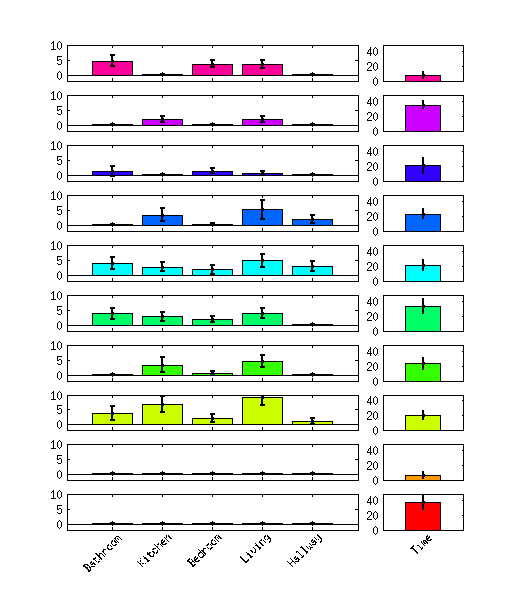
\includegraphics[width=0.45\textwidth]{Pictures/Gaus/fine/TopHN4TS48k20fine.png}\\
  a) & b)
 \end{tabular}
  \caption{House number 4, 20 topics, fine grain time, LDA-Gaussian}
\end{figure}

\begin{figure}[h!]
 \centering
 \begin{tabular}{c c}
  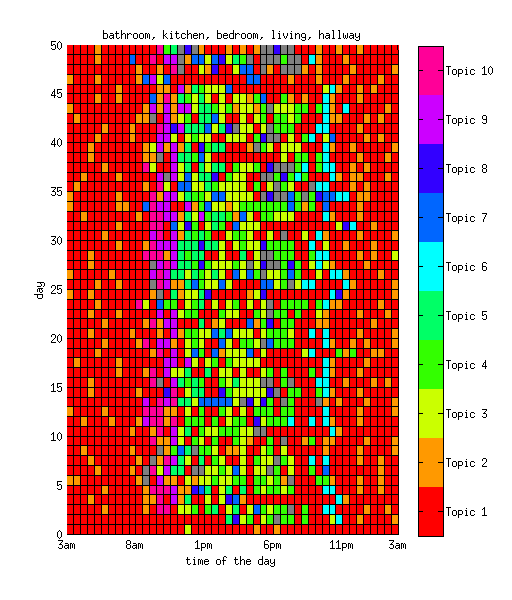
\includegraphics[width=0.45\textwidth]{Pictures/Gaus/fine/DayHN5TS48k20fine.png}
  &
  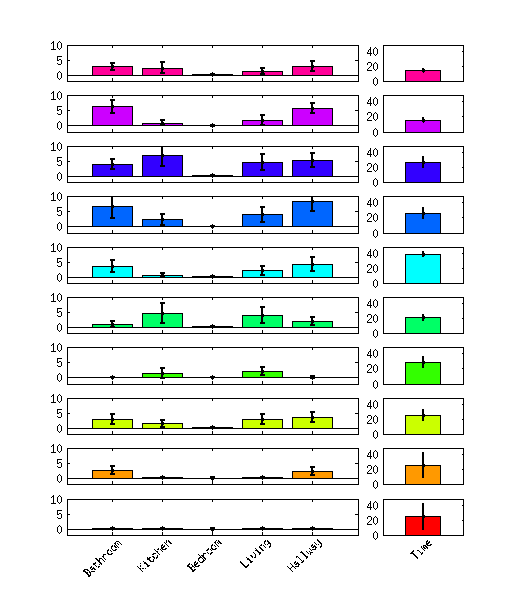
\includegraphics[width=0.45\textwidth]{Pictures/Gaus/fine/TopHN5TS48k20fine.png}\\
  a) & b)
 \end{tabular}
  \caption{House number 5, 20 topics, fine grain time, LDA-Gaussian}
\end{figure}

\chapter{LDA-Poisson}
\label{B}
Here the results for all houses are shown for the LDA-Poisson model. The number of time-slices is $n=48$ and the number of topics is $k=20$. The time dimension has a fine grain representation.


\begin{figure}[h!]
 \centering
 \begin{tabular}{c c}
  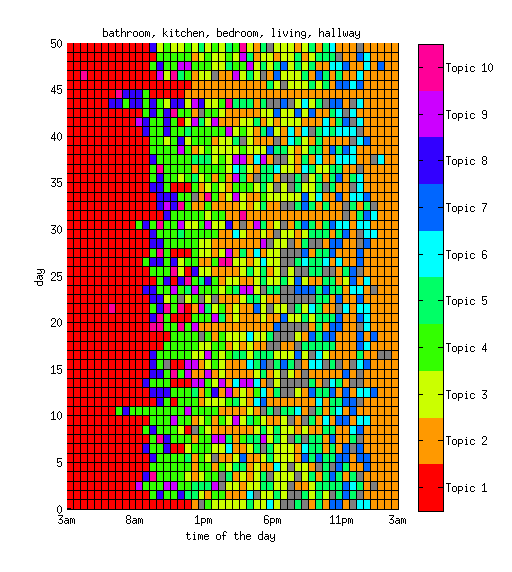
\includegraphics[width=0.45\textwidth]{Pictures/Pois/fine/DayHN1TS48k20fine.png}
  &
  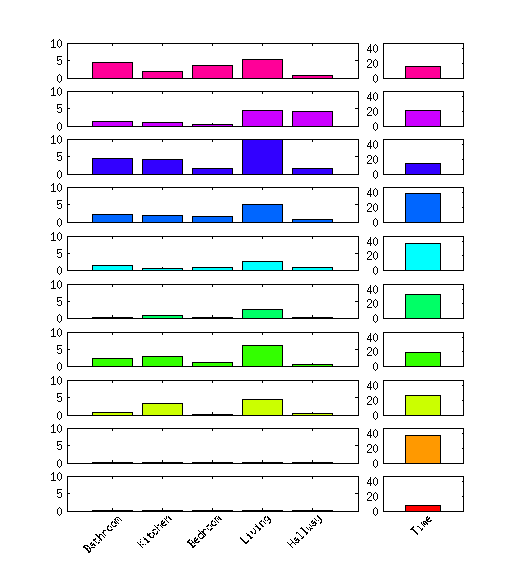
\includegraphics[width=0.45\textwidth]{Pictures/Pois/fine/TopHN1TS48k20fine.png}\\
  a) & b)
 \end{tabular}
  \caption{House number 1, 20 topics, fine grain time, LDA-Poisson}
\end{figure}

\begin{figure}[h!]
 \centering
 \begin{tabular}{c c}
  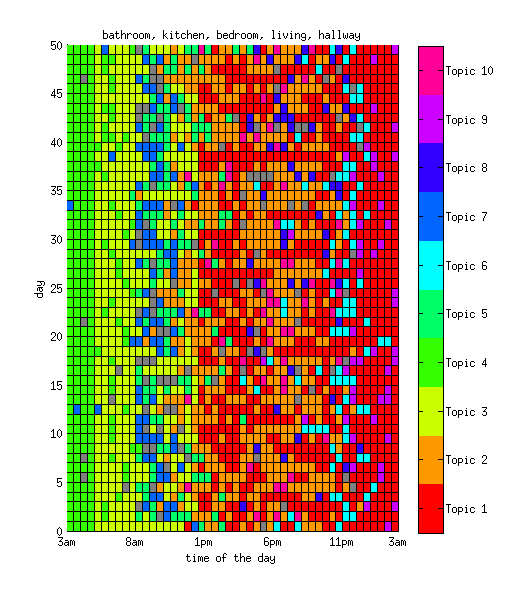
\includegraphics[width=0.45\textwidth]{Pictures/Pois/fine/DayHN2TS48k20fine.png}
  &
  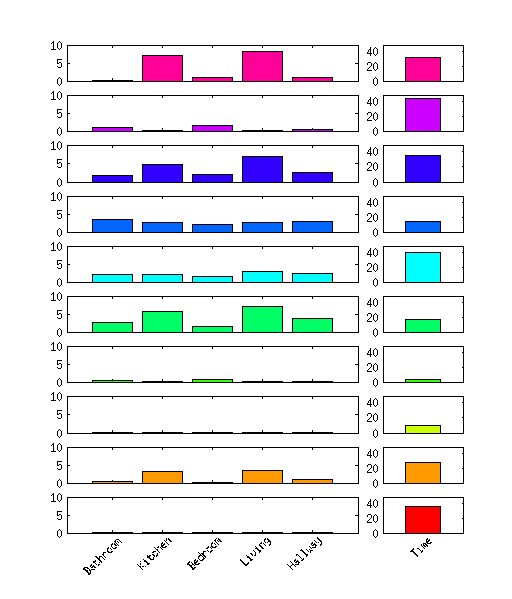
\includegraphics[width=0.45\textwidth]{Pictures/Pois/fine/TopHN2TS48k20fine.png}\\
  a) & b)
 \end{tabular}
  \caption{House number 2, 20 topics, fine grain time, LDA-Poisson}
\end{figure}

\begin{figure}[h!]
 \centering
 \begin{tabular}{c c}
  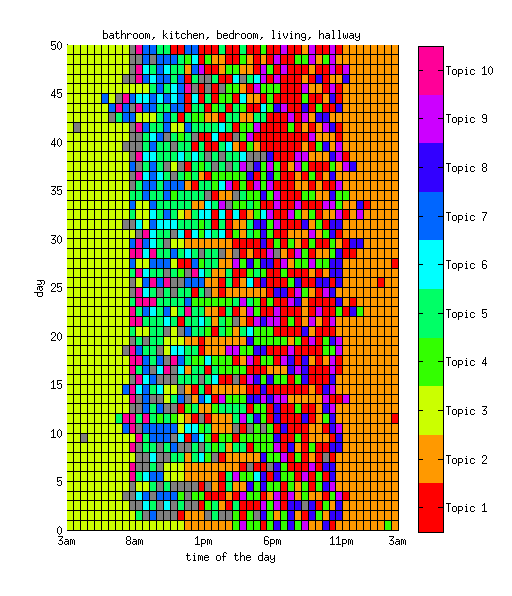
\includegraphics[width=0.45\textwidth]{Pictures/Pois/fine/DayHN3TS48k20fine.png}
  &
  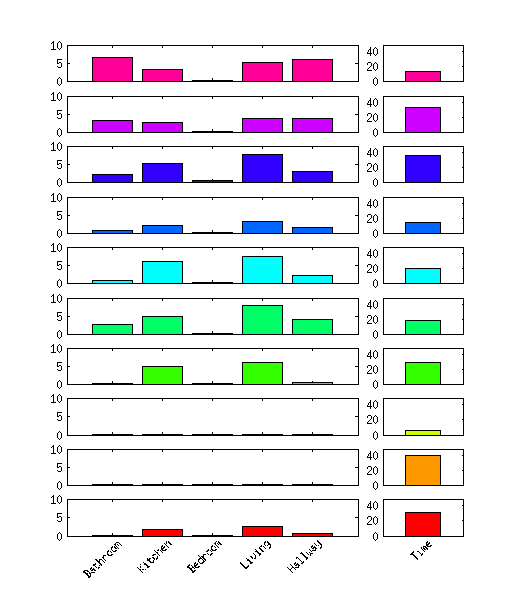
\includegraphics[width=0.45\textwidth]{Pictures/Pois/fine/TopHN3TS48k20fine.png}\\
  a) & b)
 \end{tabular}
  \caption{House number 3, 20 topics, fine grain time, LDA-Poisson}
\end{figure}

\begin{figure}[h!]
 \centering
 \begin{tabular}{c c}
  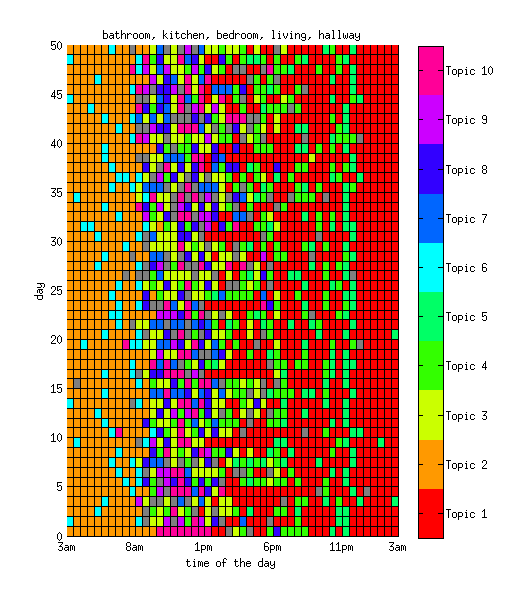
\includegraphics[width=0.45\textwidth]{Pictures/Pois/fine/DayHN4TS48k20fine.png}
  &
  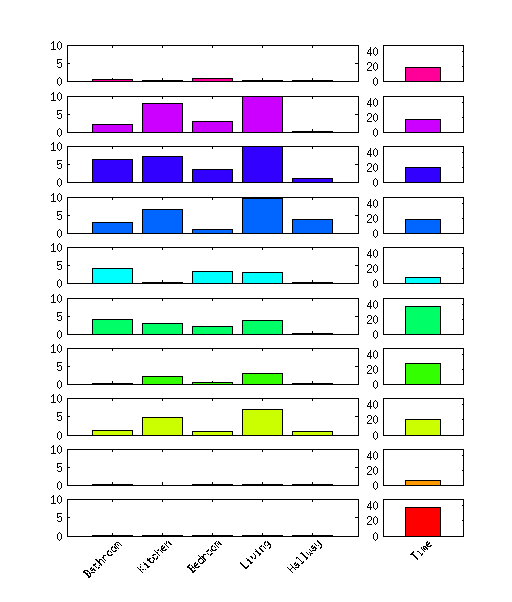
\includegraphics[width=0.45\textwidth]{Pictures/Pois/fine/TopHN4TS48k20fine.png}\\
  a) & b)
 \end{tabular}
  \caption{House number 4, 20 topics, fine grain time, LDA-Poisson}
\end{figure}

\begin{figure}[h!]
 \centering
 \begin{tabular}{c c}
  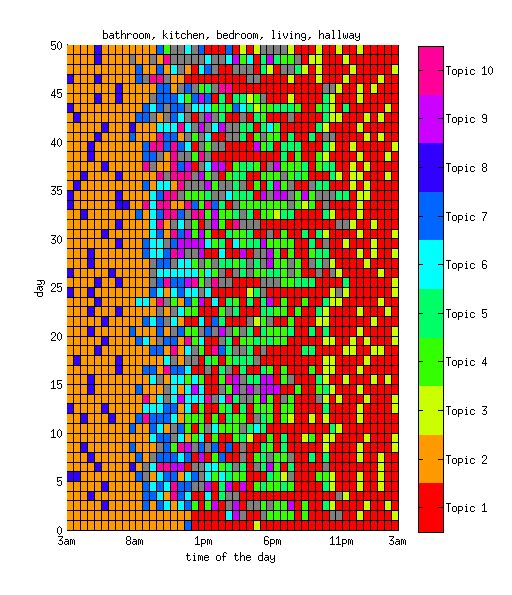
\includegraphics[width=0.45\textwidth]{Pictures/Pois/fine/DayHN5TS48k20fine.png}
  &
  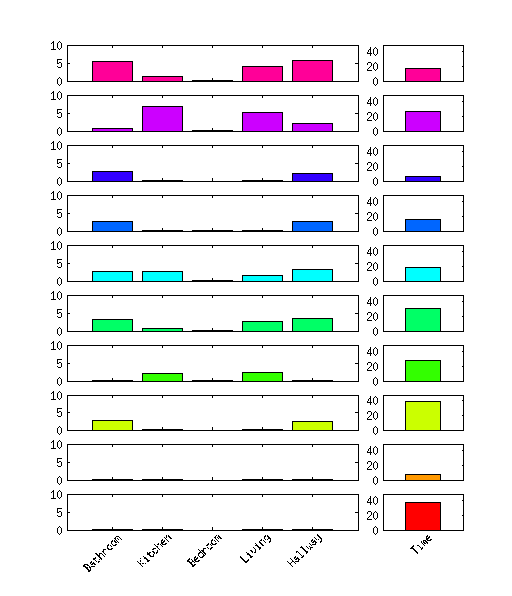
\includegraphics[width=0.45\textwidth]{Pictures/Pois/fine/TopHN5TS48k20fine.png}\\
  a) & b)
 \end{tabular}
  \caption{House number 5, 20 topics, fine grain time, LDA-Poisson}
\end{figure}
 
\end{document}
